% training_history.tex -- the merged training-history paper (P4 supply + P5 priming).
% Supersedes p4_supply.tex and p5_priming.tex (both retained in git history).
%
% GATE 0 (paper-craft), written before the merge draft:
%   Readers: training-dynamics, continual-learning, and data-curriculum researchers who assume
%            (a) a formed capability persists unless overwritten, (b) total exposure is the
%            quantity that matters, and (c) structured pre-pretraining data buys downstream
%            compute.
%   Denial:  what looks like erasure is a utilisation failure governed by the rate and spread of
%            continued use, and what looked like a priming benefit was an optimiser artifact;
%            the real controlled effect of early data at scale is what unstructured data
%            destroys.
%   Ping:    training history decides the fate of a learned capability through two levers, both
%            invisible to standard instruments: after formation, near-every-step supervised
%            contact keeps the circuit; before formation, structure in early data decides
%            whether the target remains learnable at all.
%   Nugget:  the two tells. Read-side accuracy stays at 1.000 through every collapse (the loss
%            is routing, not storage), and the structure-free control "saved more compute" than
%            the treatment (the baseline had to be broken, and it was: warmup, factor 4.19).
%   ABT:     Small transformers form an in-context binding capability under supervision, AND the
%            usual assumptions are that a formed capability persists and that structured early
%            data helps. BUT fate tracks a small continuous rate of use (identical totals fail
%            as a burst), and with warmup equalised no priming dose is compute-positive while a
%            large structure-free dose prevents learning entirely. THEREFORE the levers that
%            decide a capability's future sit in the training schedule and the structure of
%            early data, and neither behavioural monitoring nor distributional data filters can
%            see them.
%
% STATUS: merged from two campaign drafts whose every number carries a provenance row in the
% appendix. Headline numbers are numbers.tex macros regenerated by analysis/make_numbers.py
% from committed result JSONs; campaign-document numbers keep their document rows.

\documentclass[10pt]{article}
\pdfoutput=1
\usepackage[margin=1.1in]{geometry}
\usepackage{amsmath}
\usepackage{graphicx}
\usepackage[hyphens]{url}
\usepackage{tikz}
\usetikzlibrary{arrows.meta, positioning}
% GENERATED by analysis/make_numbers.py -- DO NOT EDIT.
% Every value below is computed from a committed file in paper/results/.
% If a paper types a literal instead of using these macros, verify.py will not protect it.

\newcommand{\KstarMin}{3}               % capacity_stats.json -- min k* among measurable models
\newcommand{\KstarMax}{24}               % capacity_stats.json -- censored ceiling
\newcommand{\KstarRangeFactor}{8}       % capacity_stats.json -- 8x, NOT 12x
\newcommand{\NModels}{29}                % capacity_stats.json -- after excluding pythia-70m
\newcommand{\NFamilies}{10}              % capacity_stats.json
\newcommand{\KstarOldMed}{3}            % capacity_stats.json
\newcommand{\KstarModMed}{16}            % capacity_stats.json
\newcommand{\KstarFamCI}{[+10,\,+13]}             % capacity_stats.json -- family-clustered
\newcommand{\KstarFamP}{0.012}              % capacity_stats.json
\newcommand{\PackFamP}{0.010}               % capacity_stats.json
\newcommand{\DdimFamCI}{[-0.003,\,+11.77]}              % capacity_stats.json -- touches zero -- does NOT survive
\newcommand{\OffdiagFamCI}{[-0.63,\,+0.013]}           % capacity_stats.json -- touches zero -- does NOT survive
\newcommand{\DbindFamP}{0.114}              % capacity_stats.json -- does NOT survive
\newcommand{\OffdiagFamP}{0.038}            % capacity_stats.json -- does NOT survive
\newcommand{\KstarModelP}{4.8\times 10^{-4}}            % capacity_stats.json -- model-level Mann-Whitney -- the UNclustered p
\newcommand{\NOldModels}{17}             % capacity_stats.json -- old-recipe models AFTER excluding pythia-70m
\newcommand{\NModernModels}{12}          % capacity_stats.json -- modern-recipe models
\newcommand{\NCensored}{3}              % capacity_stats.json -- right-censored at the entity-pool ceiling
\newcommand{\PackOldMed}{0.134}             % capacity_stats.json
\newcommand{\PackModMed}{0.462}             % capacity_stats.json
\newcommand{\PackFamCI}{[+0.279,\,+0.473]}              % capacity_stats.json -- family-clustered -- SURVIVES, but tautological
\newcommand{\DdimOldMed}{24.86}             % capacity_stats.json
\newcommand{\DdimModMed}{33.23}             % capacity_stats.json
\newcommand{\OffdiagOldMed}{0.388}          % capacity_stats.json
\newcommand{\OffdiagModMed}{0.183}          % capacity_stats.json
\newcommand{\OffdiagFamCITab}{[-0.629,\,+0.013]}        % capacity_stats.json -- 3 dp, p3 table column
\newcommand{\QwenLadder}{3\to10\to24\to16}             % capacity_stats.json -- 0.5B/1.5B/3B/7B -- NOT monotone, reported unsmoothed
\newcommand{\RfinalFirst}{0.194}            % capacity_control.json
\newcommand{\RfinalLast}{0.384}             % capacity_control.json
\newcommand{\RfinalChanceX}{9.6}          % capacity_control.json -- x 1/|V| (25-way)
\newcommand{\Dblock}{256}                 % capacity_control.json -- distractor tokens between declarations and query
\newcommand{\RfinalPresent}{0.167}          % capacity_control.json -- 1/K present-set baseline, K=6
\newcommand{\RfinalPresentX}{2.3}         % capacity_control.json -- x 1/K present-set
\newcommand{\Chance}{0.040}                 % capacity_control.json -- 25-way
\newcommand{\SepLast}{0.317}                % capacity_control.json
\newcommand{\SepRho}{1.000}                 % capacity_control.json
\newcommand{\SepPexact}{4.0\times 10^{-4}}              % exact_stats -- n=7; floor 2/7!
\newcommand{\SepN}{7}                   % capacity_control.json
\newcommand{\GapN}{14}                   % rigor_seeds.json -- gap-measurable; 2 censored by ceiling
\newcommand{\CertN}{16}                  % rigor_seeds.json -- all models -- cert is an AUROC over all test trials
\newcommand{\CensoredN}{2}              % rigor_seeds.json -- too few failures to measure pAcc|wrong
\newcommand{\Present}{0.125}                % rigor_seeds.json -- 1/K, K=8
\newcommand{\GapMedian}{0.29}              % rigor_seeds.json -- median pAcc|wrong
\newcommand{\GapMax}{0.65}                 % rigor_seeds.json
\newcommand{\GapMaxModel}{OPT-1.3B}            % rigor_seeds.json -- was Pythia-1.4B under the retired table
\newcommand{\GapPosSeeds}{12, 11, 12}            % rigor_seeds.json -- UNSTABLE across seeds
\newcommand{\GapPosMin}{11}              % rigor_seeds.json
\newcommand{\GapPosMax}{12}              % rigor_seeds.json
\newcommand{\GapSignP}{0.057}               % exact_stats -- worst seed
\newcommand{\GapMean}{+0.196}                % rigor_seeds.json -- clustered on model -- THIS carries the claim
\newcommand{\GapCI}{[+0.101, +0.296]}                  % rigor_seeds.json
\newcommand{\GapPos}{12}                 % rigor_seeds.json -- on seed-means, of GapN
\newcommand{\GapPosP}{0.013}                % exact_stats
\newcommand{\CertPosSeeds}{15, 12, 12}           % rigor_seeds.json -- UNSTABLE across seeds
\newcommand{\CertMean}{+0.079}               % rigor_seeds.json -- CI excludes 0
\newcommand{\CertCI}{[+0.036, +0.126]}                 % rigor_seeds.json
\newcommand{\CertPos}{13}                % rigor_seeds.json -- of 16
\newcommand{\CertSignP}{0.021}              % exact_stats
\newcommand{\EntMean}{+0.025}                % rigor_seeds.json -- CI STRADDLES 0 -- no advantage
\newcommand{\EntCI}{[-0.025, +0.078]}                  % rigor_seeds.json
\newcommand{\EntPos}{9}                 % rigor_seeds.json -- of 16
\newcommand{\EntSignP}{0.804}               % exact_stats
\newcommand{\SelfConsMean}{+0.065}           % rigor_seeds.json -- CI excludes 0
\newcommand{\SelfConsCI}{[+0.015, +0.117]}             % rigor_seeds.json
\newcommand{\SelfConsPos}{12}            % rigor_seeds.json -- of 16
\newcommand{\SelfConsSignP}{0.077}          % exact_stats
\newcommand{\RawProbeMean}{+0.003}           % rigor_seeds.json -- CI STRADDLES 0 -- no advantage
\newcommand{\RawProbeCI}{[-0.017, +0.024]}             % rigor_seeds.json
\newcommand{\RawProbePos}{8}            % rigor_seeds.json -- of 16
\newcommand{\RawProbeSignP}{1.000}          % exact_stats
\newcommand{\RawProbeNeg}{8}            % rigor_seeds.json -- loses on; of CertN
\newcommand{\CfMin}{0.11}                  % rigor_seeds.json
\newcommand{\CfMax}{0.98}                  % rigor_seeds.json
\newcommand{\NTrials}{600}                % rigor_seeds.json
\newcommand{\NSeeds}{3}                 % rigor_seeds.json
\newcommand{\CfPos}{15}                  % rigor_seeds.json -- of 16, above 0.125
\newcommand{\CfSignP}{5.2\times 10^{-4}}                % exact_stats -- the one per-model tally that clears Bonferroni (reviewer-sim fix)
\newcommand{\SteerN}{8}                 % dynamics/steer_*/steer.json
\newcommand{\SteerPos}{8}               % dynamics/steer_*/steer.json
\newcommand{\SteerMean}{+0.168}              % dynamics/steer_*/steer.json
\newcommand{\SteerSignP}{0.008}             % exact_stats
\newcommand{\RepairN}{6}                % repair_6models.json
\newcommand{\RepairPos}{5}              % repair_6models.json
\newcommand{\RepairMean}{+0.20}             % repair_6models.json
\newcommand{\RepairMax}{+0.41}              % repair_6models.json
\newcommand{\RepairSignP}{0.219}            % exact_stats -- count is WEAK
\newcommand{\RandCtrlBase}{0.22}           % repair_6models.json
\newcommand{\RandCtrlAfter}{0.10}          % repair_6models.json -- random injection HARMS
\newcommand{\LoopN}{6}                  % repair_6models.json
\newcommand{\LoopPos}{5}                % repair_6models.json
\newcommand{\LoopMean}{+0.20}               % repair_6models.json -- certificate-gated, label-free
\newcommand{\LoopHeadroomN}{5}          % repair_6models.json -- models where the ungated repair helps
\newcommand{\LoopFracMin}{83\%}            % repair_6models.json -- min share of the ungated repair's recovery captured
\newcommand{\LoopBeatsOracle}{3}        % repair_6models.json -- gated recovery >= the ungated repair's
\newcommand{\LoopCeilGated}{-0.02}          % repair_6models.json -- ceiling model, gated loop
\newcommand{\LoopCeilOracle}{-0.05}         % repair_6models.json -- ceiling model, ungated repair
\newcommand{\RepairSeeds}{3}            % repair_seeds.json
\newcommand{\RepairMeanSeeds}{+0.205}        % repair_seeds.json
\newcommand{\RepairCI}{[+0.202,\,+0.208]}               % repair_seeds.json -- seed-clustered, only 3 clusters
\newcommand{\RepairCIModel}{[+0.076,\,+0.331]}          % repair_seeds.json -- model-clustered bootstrap (6 clusters), deterministic seed
\newcommand{\RepairCtrlModelK}{6}       % repair_seeds.json -- models whose mean random-control shift is negative
\newcommand{\RepairCtrlModelN}{6}       % repair_seeds.json
\newcommand{\RepairCtrlModelP}{0.031}       % exact_stats -- model-clustered sign test -- the generalization claim
\newcommand{\RepairHelpsK}{15}           % repair_seeds.json
\newcommand{\RepairHelpsN}{18}           % repair_seeds.json
\newcommand{\RepairHelpsP}{0.0075}           % exact_stats
\newcommand{\RepairCtrlK}{18}            % repair_seeds.json
\newcommand{\RepairCtrlN}{18}            % repair_seeds.json
\newcommand{\RepairCtrlP}{7.6\times 10^{-6}}            % exact_stats -- the identification, 18/18
\newcommand{\RepairCtrlShift}{-0.096}        % repair_seeds.json
\newcommand{\AccFirst}{0.144}               % qgeom_dev.json
\newcommand{\AccLast}{0.707}                % qgeom_dev.json
\newcommand{\AccRho}{+1.000}                 % qgeom_dev.json
\newcommand{\AccP}{4.0\times 10^{-4}}                   % exact_stats -- monotone
\newcommand{\RdAccFirst}{0.171}             % qgeom_dev.json
\newcommand{\RdAccLast}{0.596}              % qgeom_dev.json
\newcommand{\RdAccRho}{+1.000}               % qgeom_dev.json
\newcommand{\RdAccP}{4.0\times 10^{-4}}                 % exact_stats
\newcommand{\CmFirst}{0.111}                % qgeom_dev.json
\newcommand{\CmLast}{0.629}                 % qgeom_dev.json
\newcommand{\CmRho}{+1.000}                  % qgeom_dev.json
\newcommand{\CmP}{4.0\times 10^{-4}}                    % exact_stats -- the fair, label-matched comparator
\newcommand{\RndNullFirst}{0.059}           % qgeom_dev.json
\newcommand{\RndNullLast}{0.272}            % qgeom_dev.json
\newcommand{\RndNullRho}{+0.857}             % qgeom_dev.json
\newcommand{\RndNullP}{0.02}               % exact_stats -- the null rises too
\newcommand{\AccGapFirst}{-0.027}            % qgeom_dev.json
\newcommand{\AccGapLast}{0.111}             % qgeom_dev.json
\newcommand{\AccGapRho}{+0.964}              % qgeom_dev.json
\newcommand{\AccGapP}{2.8\times 10^{-3}}                % exact_stats -- full - readout_k; monotone on the corrected instrument
\newcommand{\RdCmFirst}{0.060}              % qgeom_dev.json
\newcommand{\RdCmLast}{-0.033}               % qgeom_dev.json
\newcommand{\RdCmRho}{-0.893}                % qgeom_dev.json
\newcommand{\RdCmP}{0.01}                  % exact_stats -- the readout is OUTGROWN
\newcommand{\AlignFirst}{0.091}             % qgeom_dev.json
\newcommand{\AlignLast}{0.137}              % qgeom_dev.json
\newcommand{\AlignRho}{+0.429}               % qgeom_dev.json
\newcommand{\AlignP}{0.35}                 % exact_stats -- FLAT: the aim never improves
\newcommand{\AccCkpts}{7}               % qgeom_dev.json
\newcommand{\AccLayer}{12}               % qgeom_dev.json -- held fixed
\newcommand{\AccKMin}{13}                % qgeom_dev.json -- k is recomputed per checkpoint
\newcommand{\AccKMax}{27}                % qgeom_dev.json
\newcommand{\AlignNullMin}{0.0063}           % qgeom_dev.json -- k/d varies with k
\newcommand{\AlignNullMax}{0.0132}           % qgeom_dev.json
\newcommand{\AlignRatioMin}{8.8}          % qgeom_dev.json
\newcommand{\AlignRatioMax}{14.3}          % qgeom_dev.json
\newcommand{\AlignRatioMean}{11}         % qgeom_dev.json -- NOT 14x; that was the leak
\newcommand{\RdBelowCm}{3}              % qgeom_dev.json -- of AccCkpts
\newcommand{\DevReprFirst}{0.179}           % devsweep.json -- 1.4B representation clock, chance 0.040
\newcommand{\DevReprLast}{0.762}            % devsweep.json -- was hand-typed 0.712
\newcommand{\DevReadoutFirst}{0.154}        % devsweep.json -- 1.4B readout clock, chance 1/6
\newcommand{\DevReadoutLast}{0.338}         % devsweep.json -- was hand-typed 0.323
\newcommand{\DevReprXchance}{19}         % devsweep.json -- 1.4B repr LAST in units of its chance
\newcommand{\DevReadoutXchance}{2.0}      % devsweep.json -- 1.4B readout LAST in units of its chance
\newcommand{\DevNSizes}{5}              % devsweep.json -- 160M/410M/1B/1.4B/6.9B (2.8B excluded, broken revisions)
\newcommand{\DevReprXFirst}{3.1}          % devsweep.json -- smallest model
\newcommand{\DevReprXLast}{12.1}           % devsweep.json -- largest model
\newcommand{\DevReadoutXFirst}{0.9}       % devsweep.json
\newcommand{\DevReadoutXLast}{1.8}        % devsweep.json
\newcommand{\DevReadLeadsK}{5}          % devsweep.json -- sizes where repr outruns readout
\newcommand{\DevReadLeadsN}{5}          % devsweep.json
\newcommand{\RlN}{7}                    % rl_legibility/rotation_test.json -- GRPO checkpoints
\newcommand{\RlFrozenFirst}{0.864}          % rl_legibility/rotation_test.json -- frozen probe, base
\newcommand{\RlFrozenLast}{0.714}           % rl_legibility/rotation_test.json -- frozen probe, last step
\newcommand{\RlRefitFirst}{0.864}           % rl_legibility/rotation_test.json -- refit probe, base
\newcommand{\RlRefitLast}{0.792}            % rl_legibility/rotation_test.json -- refit probe, last step
\newcommand{\RlFrozenRho}{-1.000}            % rl_legibility/rotation_test.json -- frozen decays monotonically
\newcommand{\RlFrozenP}{4.0\times 10^{-4}}              % exact_stats -- n=7; floor 2/7!
\newcommand{\RlRefitRho}{-0.893}             % rl_legibility/rotation_test.json -- refit decays less
\newcommand{\RlRefitP}{0.012}               % exact_stats
\newcommand{\RlFrozenLoss}{0.150}           % rl_legibility/rotation_test.json -- a fixed readout loses this
\newcommand{\RlRefitLoss}{0.072}            % rl_legibility/rotation_test.json -- an adaptive readout loses only this
\newcommand{\CuseN}{7}                  % dynamics/em_step*/steer.json -- pretraining checkpoints
\newcommand{\CuseFirst}{0.019}              % dynamics/em_step*/steer.json -- decoded repair on failures, earliest ckpt
\newcommand{\CuseLast}{0.668}               % dynamics/em_step*/steer.json -- decoded repair on failures, final ckpt
\newcommand{\CuseRho}{+0.964}                % dynamics/em_step*/steer.json -- rises with training
\newcommand{\CuseP}{2.8\times 10^{-3}}                  % exact_stats
\newcommand{\CuseRandLast}{0.077}           % dynamics/em_step*/steer.json -- matched-norm WRONG direction barely repairs
\newcommand{\CuseBigN}{7}               % dynamics/em_step*_p69/steer.json -- 6.9B pretraining checkpoints
\newcommand{\CuseBigFirst}{0.158}           % dynamics/em_step*_p69/steer.json -- 6.9B decoded repair on failures, earliest ckpt
\newcommand{\CuseBigLast}{0.511}            % dynamics/em_step*_p69/steer.json -- 6.9B decoded repair on failures, final ckpt
\newcommand{\CuseBigRho}{+0.929}             % dynamics/em_step*_p69/steer.json -- rises with training at 6.9B
\newcommand{\CuseBigP}{6.7\times 10^{-3}}               % exact_stats
\newcommand{\DevBigProbeFirst}{0.058}       % dynamics/dev_p69/dev.json -- 6.9B best-layer decode, earliest ckpt
\newcommand{\DevBigProbeLast}{0.550}        % dynamics/dev_p69/dev.json -- 6.9B best-layer decode, final ckpt
\newcommand{\DevBigProbeXchance}{13.8}     % dynamics/dev_p69/dev.json -- 6.9B probe LAST in units of 0.040 chance
\newcommand{\DevBigProbeRho}{+0.893}         % dynamics/dev_p69/dev.json -- accessibility opens with training at 6.9B
\newcommand{\DevBigProbeP}{0.012}           % exact_stats
\newcommand{\DevBigBehavFirst}{0.075}       % dynamics/dev_p69/dev.json -- 6.9B behavioural acc, earliest ckpt
\newcommand{\DevBigBehavLast}{0.417}        % dynamics/dev_p69/dev.json -- 6.9B behavioural acc, final ckpt -- lags the probe
\newcommand{\DevSmallProbeLo}{0.058}        % dynamics/dev_p410/dev.json -- 410M probe stays near chance
\newcommand{\DevSmallProbeHi}{0.150}        % dynamics/dev_p410/dev.json -- 410M never develops
\newcommand{\DevSmallProbeRho}{-0.018}       % dynamics/dev_p410/dev.json -- no trend with training -- honest null
\newcommand{\DevSmallProbeP}{0.96}         % exact_stats -- n.s.
\newcommand{\LadderScales}{5}           % qgeom_ladder.json -- 4 usable ladder scales + 1.4B (qgeom_dev.json)
\newcommand{\LadderGapRhoLo}{+0.83}         % qgeom_ladder.json -- min gap rho across the ladder
\newcommand{\LadderGapRhoHi}{+0.98}         % qgeom_ladder.json -- max gap rho across the ladder
\newcommand{\LadNSixteenM}{9}           % qgeom_ladder.json -- checkpoints at 160M
\newcommand{\LadNFourTenM}{10}           % qgeom_ladder.json -- checkpoints at 410M
\newcommand{\LadNOneB}{14}               % qgeom_ladder.json -- checkpoints at 1B
\newcommand{\LadNSixNineB}{7}           % qgeom_ladder.json -- checkpoints at 6.9B
\newcommand{\LadNOneFourB}{7}           % qgeom_dev.json -- checkpoints at 1.4B
\newcommand{\LadderGapSigTotal}{5}      % qgeom_ladder.json -- usable gap-sig + 1.4B (now all 5)
\newcommand{\OutgrownSigTotal}{4}       % qgeom_ladder.json -- 160M/410M/1B + 1.4B = 4; breaks at 6.9B
\newcommand{\OutgrownOneBRho}{-0.90}        % qgeom_ladder.json -- 1B: strongest outgrown point
\newcommand{\OutgrownOneBP}{2.0\times 10^{-5}}          % qgeom_ladder.json -- exact p from json
\newcommand{\OutgrownBreakRho}{+0.36}       % qgeom_ladder.json -- 6.9B: readout KEEPS PACE
\newcommand{\OutgrownBreakP}{0.44}         % qgeom_ladder.json -- n.s.
\newcommand{\LadderCensored}{2.8B}         % qgeom_ladder.json -- duplicate-weight checkpoints (fabrication guard)
\newcommand{\LadGapRhoSixteenM}{+0.98}      % qgeom_ladder.json -- 160M gap rho
\newcommand{\LadMarRhoSixteenM}{-0.86}      % qgeom_ladder.json -- 160M readout-classmean rho
\newcommand{\LadAccRhoSixteenM}{-0.24}      % qgeom_ladder.json -- 160M accessibility rho
\newcommand{\LadAccLastSixteenM}{0.14}     % qgeom_ladder.json -- 160M accessibility, final ckpt
\newcommand{\LadGapRhoFourTenM}{+0.83}      % qgeom_ladder.json -- 410M gap rho
\newcommand{\LadMarRhoFourTenM}{-0.81}      % qgeom_ladder.json -- 410M readout-classmean rho
\newcommand{\LadAccRhoFourTenM}{+0.47}      % qgeom_ladder.json -- 410M accessibility rho
\newcommand{\LadAccLastFourTenM}{0.20}     % qgeom_ladder.json -- 410M accessibility, final ckpt
\newcommand{\LadGapRhoOneB}{+0.86}          % qgeom_ladder.json -- 1B gap rho
\newcommand{\LadMarRhoOneB}{-0.90}          % qgeom_ladder.json -- 1B readout-classmean rho
\newcommand{\LadAccRhoOneB}{+0.89}          % qgeom_ladder.json -- 1B accessibility rho
\newcommand{\LadAccLastOneB}{0.65}         % qgeom_ladder.json -- 1B accessibility, final ckpt
\newcommand{\LadGapRhoSixNineB}{+0.95}      % qgeom_ladder.json -- 6.9B gap rho
\newcommand{\LadMarRhoSixNineB}{+0.36}      % qgeom_ladder.json -- 6.9B readout-classmean rho
\newcommand{\LadAccRhoSixNineB}{+0.96}      % qgeom_ladder.json -- 6.9B accessibility rho
\newcommand{\LadAccLastSixNineB}{0.65}     % qgeom_ladder.json -- 6.9B accessibility, final ckpt
\newcommand{\LadAccSigTotal}{3}         % qgeom_ladder.json -- accessibility-sig scales: 1B,6.9B + 1.4B = 3
\newcommand{\LadStrongScales}{3}        % qgeom_ladder.json -- scales where the representation genuinely rises above 1/K
\newcommand{\LadderPresent}{0.167}          % qgeom_ladder.json -- 1/K present-set baseline, K=6 (same task as capacity_control)
\newcommand{\OlmoNfam}{2}               % olmo_dev.json -- developmental law now spans Pythia + OLMo-2 families
\newcommand{\OlmoOneBRho}{+0.851}            % olmo_dev.json -- OLMo-2-1B accessibility vs step
\newcommand{\OlmoOneBP}{8.0\times 10^{-5}}              % olmo_dev.json -- exact permutation p from json
\newcommand{\OlmoOneBXK}{2.33}             % olmo_dev.json -- OLMo-2-1B final probe / (1/K present-set)
\newcommand{\OlmoOneBN}{14}              % olmo_dev.json -- OLMo-2-1B checkpoints
\newcommand{\OlmoOneBClears}{7}         % olmo_dev.json -- late checkpoints clearing 1/K
\newcommand{\OlmoOneBClearsN}{7}        % olmo_dev.json -- late checkpoints
\newcommand{\OlmoSevenBRho}{+0.029}          % olmo_dev.json -- OLMo-2-7B accessibility vs step
\newcommand{\OlmoSevenBP}{1.00}            % olmo_dev.json -- exact permutation p from json
\newcommand{\OlmoSevenBXK}{1.20}           % olmo_dev.json -- OLMo-2-7B final probe / (1/K present-set)
\newcommand{\OlmoSevenBN}{6}            % olmo_dev.json -- OLMo-2-7B checkpoints
\newcommand{\OlmoSevenBClears}{1}       % olmo_dev.json -- late checkpoints clearing 1/K
\newcommand{\OlmoSevenBClearsN}{3}      % olmo_dev.json -- late checkpoints
\newcommand{\OlmoThirteenBRho}{+0.680}       % olmo_dev.json -- OLMo-2-13B accessibility vs step
\newcommand{\OlmoThirteenBP}{3.0\times 10^{-3}}         % olmo_dev.json -- exact permutation p from json
\newcommand{\OlmoThirteenBXK}{1.58}        % olmo_dev.json -- OLMo-2-13B final probe / (1/K present-set)
\newcommand{\OlmoThirteenBN}{17}         % olmo_dev.json -- OLMo-2-13B checkpoints
\newcommand{\OlmoThirteenBClears}{8}    % olmo_dev.json -- late checkpoints clearing 1/K
\newcommand{\OlmoThirteenBClearsN}{9}   % olmo_dev.json -- late checkpoints
\newcommand{\CruxN}{4}                  % cruxeval_binding/cruxeval_agg.json -- code models
\newcommand{\CruxEstab}{0}              % cruxeval_binding/cruxeval_agg.json -- gap established (pre-registered KILL fired)
\newcommand{\CruxKill}{triggered}               % cruxeval_binding/cruxeval_agg.json -- pre-registered KILL clause
\newcommand{\CruxInputXcLo}{12.7}          % cruxeval_binding/cruxeval_agg.json -- answer-slot decode of the given INPUT, x chance
\newcommand{\CruxInputXcHi}{16.0}          % cruxeval_binding/cruxeval_agg.json
\newcommand{\CruxOutputXcLo}{2.7}         % cruxeval_binding/cruxeval_agg.json -- answer-slot decode of the COMPUTED OUTPUT, x chance
\newcommand{\CruxOutputXcHi}{5.1}         % cruxeval_binding/cruxeval_agg.json -- surface-dominated: far below the input
\newcommand{\CruxFailLo}{7}             % cruxeval_binding/cruxeval_agg.json -- smallest per-model wrong-trial count
\newcommand{\CruxFailHi}{12}             % cruxeval_binding/cruxeval_agg.json -- largest; all below the pre-registered floor
\newcommand{\CruxFailFloor}{40}          % PREREG_cruxeval.md -- pre-registered minimum failure count
\newcommand{\BoxDeclLo}{0.54}              % boxes_binding/*/boxes.json -- probe reads the initial declaration, low
\newcommand{\BoxDeclHi}{0.87}              % boxes_binding/*/boxes.json -- high
\newcommand{\BoxTrackLo}{0.00}             % boxes_binding/*/boxes.json -- probe reads the tracked state, low
\newcommand{\BoxTrackHi}{0.29}             % boxes_binding/*/boxes.json -- high -- declaration-confounded
\newcommand{\ReadoutRho}{+0.70}             % readout_visibility.json
\newcommand{\ReadoutPexact}{0.23}          % exact_stats -- n=5, NOT significant
\newcommand{\ReadoutN}{5}               % readout_visibility.json
\newcommand{\ReadoutBeats}{4}           % readout_visibility.json -- of ReadoutN; NOT a control -- Vg is label-derived
\newcommand{\ReadoutBelowCm}{3}         % readout_visibility.json -- of ReadoutN; no systematic deficit
\newcommand{\DscReadout}{0.073}             % readout_visibility.json
\newcommand{\DscRandom}{0.062}              % readout_visibility.json -- indistinguishable
\newcommand{\DscFull}{0.247}                % readout_visibility.json
\newcommand{\DscAlign}{0.013}               % readout_visibility.json
\newcommand{\DscClassmean}{0.142}           % readout_visibility.json
\newcommand{\DscRandomHi}{0.076}            % readout_visibility.json -- readout_k falls BELOW the null's 95% upper bound
\newcommand{\ReadoutKVisLo}{0.52}          % readout_visibility.json -- readout_k, 3 visible models
\newcommand{\ReadoutKVisHi}{0.69}          % readout_visibility.json
\newcommand{\RandomKVisLo}{0.18}           % readout_visibility.json
\newcommand{\RandomKVisHi}{0.32}           % readout_visibility.json
\newcommand{\FullVisLo}{0.67}              % readout_visibility.json
\newcommand{\FullVisHi}{0.77}              % readout_visibility.json
\newcommand{\RcModels}{6}               % overnight rc -- 3 families, code + non-code
\newcommand{\RcGapLo}{0.21}                % overnight rc -- probe-on-errors
\newcommand{\RcGapHi}{0.35}                % overnight rc
\newcommand{\RcXfairLo}{5.8}              % overnight rc -- x FAIR null, one over present-set size
\newcommand{\RcXfairHi}{9.3}              % overnight rc
\newcommand{\RcRankTwoLo}{0.29}            % overnight rc -- model's OWN rank-2 recovers gold
\newcommand{\RcRankTwoHi}{0.41}            % overnight rc
\newcommand{\RcBeatsOut}{0}             % overnight rc -- of RcModels: probe does NOT beat the logits (0)
\newcommand{\RcBindRec}{5.5}              % overnight rc -- binding vs recency, on wrong trials
\newcommand{\RcPrimaryN}{5}             % realcode_binding/realcode_agg.json -- primary (non-censored) model x seed evaluations
\newcommand{\RcGapEstab}{4}             % realcode_binding/realcode_agg.json -- established evaluations of RcPrimaryN
\newcommand{\RcKill}{not triggered}                 % realcode_binding/realcode_agg.json -- pre-registered KILL clause
\newcommand{\RcKillP}{0.375}                % realcode_binding/realcode_agg.json -- KILL sign test
\newcommand{\RcDistinctN}{4}            % realcode_binding/*/realcode.json -- distinct code models with a primary evaluation
\newcommand{\RcDistinctEstab}{3}        % realcode_binding/*/realcode.json -- distinct models clearing the pre-registered 2x bar
\newcommand{\RcGapXcLo}{2.8}              % realcode_binding/*/realcode.json -- established-evaluation gap in units of probe chance, low
\newcommand{\RcGapXcHi}{3.7}              % realcode_binding/*/realcode.json -- high
\newcommand{\RcNotEstabXc}{1.9}           % realcode_binding/*/realcode.json -- best non-established model -- just misses 2x bar
\newcommand{\RcAccLo}{0.70}                % realcode_binding/*/realcode.json -- behavioural accuracy, low
\newcommand{\RcAccHi}{0.75}                % realcode_binding/*/realcode.json -- high
\newcommand{\RcProbeChance}{0.10}          % realcode_binding/*/realcode.json -- 1/|V|, kept distinct from behav 1/K
\newcommand{\RcDecClean}{0.49}             % realcode_binding/*/realcode.json -- DEC repair on the cleanest model (deepseek)
\newcommand{\RcWrongClean}{0.33}           % realcode_binding/*/realcode.json -- WRONG repair, same model -- DEC beats it there
\newcommand{\RcRecBind}{0.44}              % realcode_binding/*/realcode.json -- probe tracks executed value (max-separation model)
\newcommand{\RcRecLast}{0.08}              % realcode_binding/*/realcode.json -- vs the most-recent token
\newcommand{\RcBehavChance}{0.31}          % realcode_binding/*/realcode.json -- 1/K present-set baseline on executed code
\newcommand{\RcGapPresentXLo}{0.9}        % realcode_binding/*/realcode.json -- established gap vs 1/K present-set, low (~1x)
\newcommand{\RcGapPresentXHi}{1.2}        % realcode_binding/*/realcode.json -- established gap vs 1/K present-set, high
\newcommand{\RcStraddleEstab}{4}        % realcode_binding/*/realcode.json -- established CIs that STRADDLE the 1/K baseline
\newcommand{\RcStraddleN}{4}            % realcode_binding/*/realcode.json -- established evaluations
\newcommand{\RcRecBindMean}{0.25}          % realcode_binding/*/realcode.json -- mean binding-recovery across primary runs
\newcommand{\RcRecLastMean}{0.12}          % realcode_binding/*/realcode.json -- mean most-recent-token recovery
\newcommand{\RcRecBindLo}{0.12}            % realcode_binding/*/realcode.json -- binding-recovery range, low
\newcommand{\RcRecBindHi}{0.44}            % realcode_binding/*/realcode.json -- binding-recovery range, high
\newcommand{\RcRecBindWinK}{4}          % realcode_binding/*/realcode.json -- runs where binding beats recency (mixed: loses on 1)
\newcommand{\RcRecBindWinN}{5}          % realcode_binding/*/realcode.json -- primary runs
\newcommand{\DscSteer}{0.040}               % readout_visibility.json -- smallest of the 5
\newcommand{\CorpusN}{11,583}                % corpus_stats.json -- SWE-bench attempts, DeepSWE-v11 -- NOT gpt-oss
\newcommand{\CorpusRecallFail}{0.68}       % corpus_stats.json -- gold-file recall on failures
\newcommand{\CorpusRecallPass}{0.81}       % corpus_stats.json -- gold-file recall on passes
\newcommand{\CorpusCovFail}{0.55}          % corpus_stats.json -- edit-coverage on failures
\newcommand{\CorpusCovPass}{0.74}          % corpus_stats.json -- edit-coverage on passes
\newcommand{\CorpusSawNeverEdited}{27}   % corpus_stats.json -- % of failures: opened a gold file, never edited it
\newcommand{\CorpusEditedAllFail}{10.7}    % corpus_stats.json -- % edited every gold file, still failed
\newcommand{\CorpusOmissionShare}{53}    % corpus_stats.json -- % of failures that are omission
\newcommand{\CorpusWrongLogicShare}{21}  % corpus_stats.json -- % wrong logic, the comparator
\newcommand{\CorpusApiShare}{55}         % corpus_stats.json -- % modal failing construct: api-interface wiring
\newcommand{\GossSolveBare}{0.128}          % gptoss_g1_forensics.json -- gpt-oss-20B G1 run 1 (bare greedy)
\newcommand{\GossSolveFixed}{0.300}         % gptoss_g1_forensics.json -- run 2 (temp 1.0 + retry)
\newcommand{\GossNeverEditBare}{61}      % gptoss_g1_forensics.json -- % episodes never emitting an edit, run 1
\newcommand{\GossNeverEditFixed}{28}     % gptoss_g1_forensics.json -- % never-edit after sampling fix
\newcommand{\GossLocateEditRatio}{42}    % gptoss_g1_forensics.json -- locate:edit tool-call ratio, run 1
\newcommand{\GossSolveAmongEdited}{0.42}   % gptoss_g1_forensics.json -- solve rate among episodes that DID edit
\newcommand{\GossPaccWrong}{0.73}          % figdata.json -- gpt-oss-20B probe decode on its wrong trials
\newcommand{\GossRepairBase}{0.942}         % figdata.json -- gpt-oss-20B base recall, repair battery
\newcommand{\GossRepairReinj}{0.978}        % figdata.json -- after re-injecting its own decoded binding
\newcommand{\GossRepairCtrl}{0.523}         % figdata.json -- after format-matched WRONG content -- harms
\newcommand{\OlmoGapBase}{0.58}            % figdata.json -- OLMo-2-7B base pAcc|wrong
\newcommand{\OlmoGapInstr}{0.60}           % figdata.json -- OLMo-2-7B-Instruct pAcc|wrong -- alignment does not close the gap
\newcommand{\DdeclPearson}{+0.64}           % figdata.json -- k* vs entity-code dimension, model level
\newcommand{\DdeclSpearman}{+0.77}          % figdata.json -- rank version
\newcommand{\OffdiagPearson}{-0.52}         % figdata.json -- k* vs interference, model level
\newcommand{\DdeclPartial}{+0.54}           % figdata.json -- k* vs entity-code dimension, controlling interference -- n=29, was 0.56 at n=30
\newcommand{\OffdiagPartial}{-0.34}         % figdata.json -- k* vs interference, controlling dimension -- n=29, was -0.35 at n=30
\newcommand{\QueryDecodeN}{5}           % qgx2/*/qgeom.json -- models with a committed query-site decode
\newcommand{\QueryDecodeLo}{0.51}          % qgx2/*/qgeom.json -- retrieved obligation at the QUERY site, weakest model
\newcommand{\QueryDecodeHi}{0.86}          % qgx2/*/qgeom.json -- strongest -- vs 0.017-0.054 at the declaration site
\newcommand{\NModelsRaw}{30}             % figdata.json -- models in the RAW table, BEFORE excluding pythia-70m
\newcommand{\NOldRaw}{18}                % figdata.json -- old-recipe rows, raw table
\newcommand{\NModernRaw}{12}             % figdata.json -- modern-recipe rows, raw table
\newcommand{\PythiaLadder}{3,4,6,4,4}           % figdata.json -- k* at 410M/1.4B/2.8B/6.9B/12B -- FLAT
\newcommand{\PythiaKstarLo}{3}          % figdata.json
\newcommand{\PythiaKstarHi}{6}          % figdata.json
\newcommand{\PythiaKstarFirst}{3}       % figdata.json -- 410M
\newcommand{\PythiaKstarLast}{4}        % figdata.json -- 12B -- 29x the parameters, +1 binding
\newcommand{\KstarOlmoE}{6}             % figdata.json -- a MODERN model low in the range -- the classes overlap
\newcommand{\KstarOptOneThree}{10}       % figdata.json -- an OLD model high in the range
\newcommand{\KstarOlmoLadder}{16}        % figdata.json -- base/SFT/DPO/Instruct -- identical at every stage
\newcommand{\PythiaSeventyCeiling}{0.070}   % figdata.json -- K=1 ceiling of the EXCLUDED model, vs 0.040 chance
\newcommand{\PythiaSeventyKstar}{2}     % figdata.json -- not a measurement -- its K=1 ceiling is at chance
\newcommand{\RobustN}{8}                % figdata.json -- models with committed D-sweep curves
\newcommand{\RobustK}{8}                % figdata.json -- K held fixed while D varies
\newcommand{\TransferN}{6}              % figdata.json -- models in the zero-shot transfer battery
\newcommand{\TransferPureK}{6}          % figdata.json -- positive on ALL THREE single-axis shifts
\newcommand{\TransferComboK}{5}         % figdata.json -- still positive when shifts stack (OLMoE drops out)
\newcommand{\HtHN}{7}                   % headtohead_stats.json -- models in the positional head-to-head
\newcommand{\HtHPosAurocLo}{0.593}          % headtohead_stats.json -- positional model, weakest
\newcommand{\HtHPosAurocHi}{0.843}          % headtohead_stats.json -- positional model, strongest
\newcommand{\HtHIncLo}{-0.0005}               % headtohead_stats.json -- overlap's increment, low
\newcommand{\HtHIncHi}{+0.0048}               % headtohead_stats.json -- overlap's increment, high -- adds nothing
\newcommand{\HtHFoilOvlLo}{0.12}           % headtohead_stats.json -- emitted foil = max-overlap competitor, low
\newcommand{\HtHFoilOvlHi}{0.19}           % headtohead_stats.json -- at or below the 0.20 chance
\newcommand{\HtHFoilOvlChance}{0.20}       % headtohead_stats.json
\newcommand{\PosVarOlmo}{0.23}             % dynamics/geo_*/geom.json -- OLMo-2 is the ONE model where position does not dominate
\newcommand{\DcovQsevenB}{1.3}            % dynamics/geo_*/geom.json -- covariance PR, Qwen2.5-7B -- the ARTIFACT
\newcommand{\TopOneQsevenB}{54}          % dynamics/geo_*/geom.json -- % of residual variance in ONE coordinate
\newcommand{\DdimQonefiveB}{12.0}          % dynamics/geo_*/geom.json -- standardized PR, Qwen2.5-1.5B
\newcommand{\DdimQsevenB}{35.3}            % dynamics/geo_*/geom.json -- standardized PR, Qwen2.5-7B -- the CORRECTED estimate
\newcommand{\DdimQfourteenB}{81.1}         % dynamics/geo_*/geom.json -- standardized PR, Qwen2.5-14B -- scales with size
\newcommand{\PosVarDevFirst}{0.15}         % dynamics/geo_*/geom.json -- Pythia-1.4B step 1000
\newcommand{\PosVarDevLast}{0.99}          % dynamics/geo_*/geom.json -- step 143000 -- the confound is LEARNED
\newcommand{\TopOneDevFirst}{0.001}         % dynamics/geo_*/geom.json -- Pythia-1.4B step 1000
\newcommand{\TopOneDevLast}{0.17}          % dynamics/geo_*/geom.json -- step 143000 -- so does the massive activation
\newcommand{\GeoNModels}{8}             % dynamics/geo_*/geom.json -- frozen models with committed declaration-site geometry
\newcommand{\GeoNNonOlmo}{7}            % dynamics/geo_*/geom.json -- excluding OLMo-2, the one exception to position dominance
\newcommand{\PosVarLoPct}{98.1}            % dynamics/geo_*/geom.json -- low end IS DeepSeek-Coder: 98.1, not the old 99.3
\newcommand{\PosVarHiPct}{99.9}            % dynamics/geo_*/geom.json
\newcommand{\PosVarOlmoPct}{23}          % dynamics/geo_*/geom.json -- OLMo-2, the one exception, in the same percent units as the range
\newcommand{\RawIntLo}{0.84}               % dynamics/geo_*/geom.json -- raw pairwise cos^2 -- it is describing position
\newcommand{\RawIntHi}{1.00}               % dynamics/geo_*/geom.json
\newcommand{\DrawHi}{1.03}                 % dynamics/geo_*/geom.json -- raw PR is ~1 wherever position dominates
\newcommand{\ResidIntLo}{0.006}             % dynamics/geo_*/geom.json -- residual interference after removing the per-slot mean
\newcommand{\ResidIntHi}{0.009}             % dynamics/geo_*/geom.json
\newcommand{\RobustLowKN}{4}            % figdata.json -- robust-sweep models with k* below the sweep's K=8
\newcommand{\RobustLowKDzeroHi}{0.38}      % figdata.json -- highest D=0 recall among the k*<8 models
\newcommand{\RobustHighKDzeroLo}{0.70}     % figdata.json -- lowest D=0 recall among the k*>=16 models
\newcommand{\RobustDmax}{256}             % figdata.json -- largest distractor block in the sweep
\newcommand{\RobustDzeroLo}{0.27}          % figdata.json -- D=0 recall, lowest of 8 -- already collapsed at K=8
\newcommand{\RobustDzeroHi}{0.96}          % figdata.json -- D=0 recall, highest of 8
\newcommand{\RobustDzeroMed}{0.54}         % figdata.json -- D=0 recall, median of 8
\newcommand{\RobustDendLo}{0.10}           % figdata.json -- D=256 recall, lowest of 8
\newcommand{\RobustDendHi}{0.31}           % figdata.json -- D=256 recall, highest of 8
\newcommand{\RobustDendMed}{0.20}          % figdata.json -- D=256 recall, median of 8
\newcommand{\SftFailBase}{194}            % rlvr_sft_stages.json -- OLMo-2-7B failures/400, base
\newcommand{\SftFailSFT}{58}             % rlvr_sft_stages.json -- failures/400 after SFT -- most of the drop is here
\newcommand{\SftFailDPO}{49}             % rlvr_sft_stages.json -- failures/400 after DPO
\newcommand{\SftFailRLVR}{48}            % rlvr_sft_stages.json -- failures/400 after RLVR -- barely moves
\newcommand{\SftProbeBase}{0.787}           % rlvr_sft_stages.json -- probe decodability, base
\newcommand{\SftProbeSFT}{0.953}            % rlvr_sft_stages.json -- probe decodability after SFT -- jumps then flat
\newcommand{\SftDdeclRLVRDelta}{-0.07}      % rlvr_sft_stages.json -- RLVR moves the declaration-site subspace by this (entity-code, not binding)
\newcommand{\SftSpearFirst}{0.367}          % rlvr_sft_stages.json -- Spearman(probe,model), base
\newcommand{\SftSpearLast}{0.667}           % rlvr_sft_stages.json -- Spearman(probe,model), post-RLVR -- posteriors converge
\newcommand{\RlStepN}{5}                % rlvr_sft_stages.json -- collision-free RL-Zero-Code step branches
\newcommand{\RlStepSpan}{2,400}             % rlvr_sft_stages.json -- RL steps spanned
\newcommand{\RlStepProbeFirst}{0.827}       % rlvr_sft_stages.json -- probe decodability, first RL step
\newcommand{\RlStepProbeLast}{0.720}        % rlvr_sft_stages.json -- probe decodability, last RL step -- falls
\newcommand{\RlStepRecallFirst}{0.590}      % rlvr_sft_stages.json -- recall @ K=10, first RL step
\newcommand{\RlStepRecallLast}{0.510}       % rlvr_sft_stages.json -- recall @ K=10, last RL step -- falls
\newcommand{\RlStepMarginFirst}{+0.310}      % rlvr_sft_stages.json -- capacity margin @ K=10, first RL step
\newcommand{\RlStepMarginLast}{-0.020}       % rlvr_sft_stages.json -- capacity margin @ K=10, last -- crosses zero
\newcommand{\RlStepDdeclLo}{68.42}          % rlvr_sft_stages.json -- declaration-site subspace dim, min over RL steps
\newcommand{\RlStepDdeclHi}{68.57}          % rlvr_sft_stages.json -- declaration-site subspace dim, max -- frozen
\newcommand{\RlStepDdeclPct}{0.1}         % rlvr_sft_stages.json -- half-range of d_decl as % -- geometry frozen (+/-0.1%)
\newcommand{\DevTrnAccFirst}{0.261}         % developmental_trn1/dev-p14b.json -- accessibility, step1000
\newcommand{\DevTrnAccLast}{0.972}          % developmental_trn1/dev-p14b.json -- accessibility, step143000
\newcommand{\DevTrnBehavLast}{0.610}        % developmental_trn1/dev-p14b.json -- behaviour, step143000
\newcommand{\DevTrnProbeOnFail}{0.953}      % developmental_trn1/dev-p14b.json -- p(probe right | model wrong), final ckpt
\newcommand{\DevTrnBaseline}{0.167}         % developmental_trn1/dev-p14b.json -- 1/K present-set baseline
\newcommand{\DevTrnGapSlope}{+0.179}         % two_clocks.json -- gap slope per log10 step, 1.4B
\newcommand{\DevTrnGapSlopeCILo}{0.126}     % two_clocks.json
\newcommand{\DevTrnGapSlopeCIHi}{0.279}     % two_clocks.json
\newcommand{\DevTrnSmallSlope}{+0.058}       % two_clocks.json -- gap slope, 410M -- n.s.
\newcommand{\DevTrnSmallSlopeCILo}{-0.051}   % two_clocks.json
\newcommand{\DevTrnSmallSlopeCIHi}{0.143}   % two_clocks.json -- CI spans zero
\newcommand{\OnsetLag}{+0.061}               % two_clocks.json -- onset lag in decades, 1.4B
\newcommand{\OnsetLagCILo}{-0.100}           % two_clocks.json
\newcommand{\OnsetLagCIHi}{0.212}           % two_clocks.json -- CI spans zero -- onset claim NOT supported
\newcommand{\CapAlpha}{0.820}               % capacity_alpha_fit.json -- K50 = c*N^alpha, D=0, uncensored
\newcommand{\CapAlphaCILo}{0.674}           % capacity_alpha_fit.json
\newcommand{\CapAlphaCIHi}{1.251}           % capacity_alpha_fit.json
\newcommand{\CapRsq}{0.73}                 % capacity_alpha_fit.json
\newcommand{\CapLofoLo}{0.76}              % capacity_alpha_fit.json -- leave-one-family-out alpha, min
\newcommand{\CapLofoHi}{1.09}              % capacity_alpha_fit.json -- leave-one-family-out alpha, max
\newcommand{\CapFitN}{11}                % capacity_alpha_fit.json -- models entering the fit
\newcommand{\TrnRecipeCoef}{+0.123}          % capacity_trn1_summary.json -- recipe coef controlling scale -- interval spans zero
\newcommand{\TrnRecipeCILo}{-0.521}          % capacity_trn1_summary.json
\newcommand{\TrnRecipeCIHi}{0.363}          % capacity_trn1_summary.json
\newcommand{\TrnScaleCoef}{+0.818}           % capacity_trn1_summary.json -- log-params coef, same regression
\newcommand{\TrnScaleCILo}{0.697}           % capacity_trn1_summary.json
\newcommand{\TrnScaleCIHi}{1.206}           % capacity_trn1_summary.json -- excludes zero
\newcommand{\TrnOptResolved}{38.1}         % capacity_trn1_summary.json -- opt-1.3b resolves past the old K=24 ceiling
\newcommand{\TrnIntRetained}{0.535}         % interference_axis.json -- median retained capacity fraction under D=256
\newcommand{\TrnIntReduced}{10}          % interference_axis.json
\newcommand{\TrnIntN}{11}                % interference_axis.json
\newcommand{\TrnIntRho}{+0.20}              % interference_axis.json -- capacity does not predict robustness
\newcommand{\TrnIntP}{0.56}                % interference_axis.json
\newcommand{\BoundMeasured}{3.7}          % cross_campaign_capacity.json -- 4.98M task-trained capacity
\newcommand{\BoundPredicted}{0.14}         % cross_campaign_capacity.json -- law prediction at 4.98M
\newcommand{\BoundFactor}{26}            % cross_campaign_capacity.json -- the regime boundary
\newcommand{\CapLooMax}{0.11}              % capacity_alpha_fit.json -- max |delta alpha| deleting any single model
\newcommand{\TimeLawHCoef}{766}           % extra_analyses.json -- t = c*K^a, H100 clocks corpus
\newcommand{\TimeLawHExp}{2.58}            % extra_analyses.json
\newcommand{\TimeLawHRsq}{0.95}            % extra_analyses.json
\newcommand{\TimeLawDCoef}{667}           % devaxis_analyses.json -- same law, Trainium codebase
\newcommand{\TimeLawDExp}{2.12}            % devaxis_analyses.json
\newcommand{\TimeLawDRsq}{0.97}            % devaxis_analyses.json
\newcommand{\TimeLawExpNoKeight}{1.7}     % devaxis_analyses.json -- devaxis exponent w/o the n=2 K=8 cell -- honest low end
\newcommand{\TimeLawDblLo}{4}           % extra_analyses.json + devaxis_analyses.json -- step-cost factor per doubling of K, low
\newcommand{\TimeLawDblHi}{6}           % extra_analyses.json + devaxis_analyses.json -- high
\newcommand{\LearnSmallN}{23}            % extra_analyses.json -- runs at 1.31M params
\newcommand{\LearnSmallEmerged}{0}      % extra_analyses.json -- none form at 1.31M in measured budgets
\newcommand{\SeedOverdisp}{9.05}           % devaxis_analyses.json -- seed variance / binomial
\newcommand{\DevaxisRuns}{1,301}            % devaxis_analyses.json -- Trainium program total
\newcommand{\GapCellUniform}{5/5}         % x14_gap_law.json -- re-formed/complete at max gap 14
\newcommand{\GapCellUniformPct}{100}      % x14_gap_law.json
\newcommand{\GapCellPeriodic}{3/11}        % x14_gap_law.json -- re-formed/complete at max gap 99
\newcommand{\GapCellPeriodicPct}{27}     % x14_gap_law.json
\newcommand{\GapCellClustered}{2/10}       % x14_gap_law.json -- re-formed/complete at max gap 990
\newcommand{\GapCellClusteredPct}{20}    % x14_gap_law.json
\newcommand{\GapCellBlocks}{1/12}          % x14_gap_law.json -- re-formed/complete at max gap 10395
\newcommand{\GapCellBlocksPct}{8}       % x14_gap_law.json
\newcommand{\GapFifty}{64}               % x14_gap_law.json -- logistic 50% point in log gap
\newcommand{\GapSpanFactor}{742}          % x14_gap_law.json -- max/min gap ratio at matched rate+totals
\newcommand{\GapIncomplete}{8}          % x14_gap_law.json -- incomplete rescues excluded and counted
\newcommand{\DzBaseN}{39}                % d250_verdict.json -- pooled baseline
\newcommand{\DzBaseCross}{38}            % d250_verdict.json
\newcommand{\DzBaseMed}{6,750}              % d250_verdict.json
\newcommand{\DzChessN}{20}               % d250_verdict.json
\newcommand{\DzChessCross}{20}           % d250_verdict.json
\newcommand{\DzChessMed}{6,375}             % d250_verdict.json
\newcommand{\DzShufCross}{17}            % d250_verdict.json
\newcommand{\DzShufCens}{3}             % d250_verdict.json
\newcommand{\DzShufMed}{9,000}              % d250_verdict.json
\newcommand{\DzPChess}{0.73}               % d250_verdict.json -- verdict NOT CONFIRMED
\newcommand{\DzPShuf}{0.002}                % d250_verdict.json -- specificity arm slows learning
\newcommand{\WuRatio}{3.89}                % h100_reanalysis.json -- re-derived warmup handicap
\newcommand{\WuP}{2.3\times10^{-7}}                    % h100_reanalysis.json
\newcommand{\WuSlowMed}{26,250}              % h100_reanalysis.json -- warmup-500 baseline median
\newcommand{\WuSlowN}{19}                % h100_reanalysis.json
\newcommand{\WuSlowCross}{19}            % h100_reanalysis.json -- crosses eventually
\newcommand{\WuFastMed}{6,750}              % h100_reanalysis.json -- warmup-free baseline median
\newcommand{\WuFastN}{33}                % h100_reanalysis.json
\newcommand{\WuFastCross}{32}            % h100_reanalysis.json
\newcommand{\SaveChessLo}{18.1}            % h100_reanalysis.json -- chess savings vs cold baseline, k-steps, min over doses
\newcommand{\SaveChessHi}{19.5}            % h100_reanalysis.json -- max
\newcommand{\SaveShufLo}{16.1}             % h100_reanalysis.json -- shuffle_chess savings vs cold baseline, k-steps, min over doses
\newcommand{\SaveShufHi}{18.9}             % h100_reanalysis.json -- max
\newcommand{\SaveRandLo}{19.4}             % h100_reanalysis.json -- chess_random savings vs cold baseline, k-steps, min over doses
\newcommand{\SaveRandHi}{19.9}             % h100_reanalysis.json -- max
\newcommand{\HarmChessFive}{9/10}          % h100_reanalysis.json -- crossing at dose 5k, warmup-matched
\newcommand{\HarmShufFive}{1/10}           % h100_reanalysis.json
\newcommand{\HarmPFive}{0.0011}              % h100_reanalysis.json
\newcommand{\HarmChessTen}{10/10}           % h100_reanalysis.json
\newcommand{\HarmShufTen}{2/10}            % h100_reanalysis.json
\newcommand{\HarmPTen}{0.0007}               % h100_reanalysis.json
\newcommand{\HarmChessTwenty}{42/45}        % h100_reanalysis.json -- dose 20k: structure survives
\newcommand{\HarmShufTwenty}{1/18}         % h100_reanalysis.json -- dose 20k: statistics-only collapses
\newcommand{\HarmPTwenty}{1.9\times10^{-11}}            % h100_reanalysis.json -- exact two-sided Fisher on the dose-20k cells
\newcommand{\SpeedChessB}{6,500}            % h100_reanalysis.json -- phase-B median after chess d5000
\newcommand{\SpeedShufB}{21,875}             % h100_reanalysis.json -- after shuffled chess d5000
\newcommand{\SpeedRatio}{3.4}             % h100_reanalysis.json
\newcommand{\SpeedShufP}{5.1\times10^{-10}}             % h100_reanalysis.json -- phase-B vs warmup-matched base
\newcommand{\SpeedChessP}{0.12}            % h100_reanalysis.json -- not significant
\newcommand{\StratChessR}{101/105}            % h100_reanalysis.json -- re-derived strategy null
\newcommand{\StratRandR}{73/78}             % h100_reanalysis.json
\newcommand{\StratP}{0.50}                 % h100_reanalysis.json
\newcommand{\RevZero}{0/11}                % h100_reanalysis.json -- revival at p=0
\newcommand{\RevTwoTh}{0/6}               % h100_reanalysis.json
\newcommand{\RevFiveTh}{3/6}              % h100_reanalysis.json
\newcommand{\RevOne}{6/6}                 % h100_reanalysis.json -- full revival from p=0.01
\newcommand{\RetKfZero}{0/21}              % devaxis_analyses.json -- K=4 retention at p=0
\newcommand{\RetKfLow}{1/7}               % devaxis_analyses.json -- K=4 at p=0.01
\newcommand{\RetKfTwo}{4/7}               % devaxis_analyses.json -- K=4 at p=0.02
\newcommand{\RetKfThree}{7/7}             % devaxis_analyses.json -- K=4 at p=0.03
\newcommand{\RetKtZero}{37/96}              % devaxis_analyses.json -- K=2 at p=0
\newcommand{\RetKtTwo}{8/8}               % devaxis_analyses.json -- K=2 at p=0.02
\newcommand{\RetKtThree}{7/8}             % devaxis_analyses.json -- K=2 at p=0.03 -- within its interval
\newcommand{\TokLawHExp}{2.67}             % token_costs.json -- time law refit in token units, H100
\newcommand{\TokLawHRsq}{0.95}             % token_costs.json
\newcommand{\TokLawDExp}{2.43}             % token_costs.json -- devaxis
\newcommand{\TokLawDRsq}{0.98}             % token_costs.json
\newcommand{\TokLawDExpNoKeight}{1.9}     % token_costs.json -- without the K=8 cell
\newcommand{\TokKfourH}{206}              % token_costs.json -- K=4 formation, millions of tokens, H100
\newcommand{\TokKfourD}{65}              % token_costs.json -- devaxis
\newcommand{\TokWindow}{69.1}              % token_costs.json -- 10k-step deprivation window, M tokens
\newcommand{\TokTrickle}{0.35}             % token_costs.json -- deciding supervised trickle, M tokens
\newcommand{\TokTricklePct}{0.5}          % token_costs.json -- trickle as % of window throughput
\newcommand{\TokGapFifty}{0.58}            % token_costs.json -- gap50 in M unsupervised tokens
\newcommand{\TokBaseReqLo}{13.9}           % token_costs.json -- task requirement, M tokens, campaign accounting
\newcommand{\TokBaseReqHi}{16.0}           % token_costs.json -- raw-record accounting
\newcommand{\TokWuWaste}{46.2}             % token_costs.json -- warmup-500 extra cost per run, M tokens
\newcommand{\TokWuWasteMult}{2.9}         % token_costs.json -- warmup waste as a multiple of the task's own requirement
\newcommand{\TokHarmDose}{47.4}            % token_costs.json -- the dose-20k structure-free corpus, M tokens

\definecolor{housetea}{HTML}{1F6F78}
\definecolor{houseclay}{HTML}{C0442E}
\title{Training history and the fate of a learned capability:\\
supervision supply, and the structure of early data}
\author{Manas Venkata Sai Ravulapalli}
\date{}

\begin{document}
\maketitle

\begin{abstract}
Two decisions in a training schedule are usually made blind: how much supervised contact a
formed capability keeps receiving, and what data the network sees before the target task
arrives. We measure both on the same in-context binding task, in small transformers
(1.3M--5M parameters), across two independent codebases on two accelerator platforms. The
corpus is \DevaxisRuns{} Trainium runs and 985 H100 farm runs, 651 priming and 230
maintenance of them re-derived from raw records. After formation, fate tracks a small
continuous rate of use. The loss under deprivation is not erasure: read-side accuracy stays
at 1.000 through every collapse while use-side accuracy falls to chance. Keeping the
capability costs 1--3\% of full supervision under the primary retention criterion. At
matched mean rate and totals, re-formation falls monotonically with the maximum unsupervised
gap: \GapCellUniformPct\% at 14 steps, \GapCellBlocksPct\% at 10{,}395, a logistic 50\%
point near a gap of \GapFifty{} steps. Revival after collapse
needs roughly ten times more supply and fails at true zero within an $8\times$ formation
budget, and models with and without a trickle through the deprivation window are
behaviourally identical at
rescue time yet recover at 31/40 vs 18/40 (McNemar $p=0.0072$); at true zero the collapsed
network is worse at rebuilding the task than a fresh initialisation. Before formation, the
apparent benefit of structured priming was an optimiser artifact: an unprimed baseline pays
a factor of about four for a standard learning-rate warmup, so every substrate ``helps,''
including the structure-free control. With warmup equalised, no dose is established as
compute-positive (a candidate low-dose acceleration did not survive a pre-registered
replication, $p=\DzPChess$ at $n=\DzChessN$), and what survives is harm: at dose 20{,}000,
priming with destroyed structure but identical token statistics nearly abolishes learning
(\HarmShufTwenty{} vs \HarmChessTwenty{} crossing, exact Fisher $p=\HarmPTwenty$). Training
history acts through two levers, and the instruments that usually guard a pipeline,
behavioural monitoring and distributional data filters, see neither.
\end{abstract}

\section{Introduction}

A capability that a network acquired under supervision can be lost when that supervision
thins, and a network's later learning can be helped or hurt by what it saw first. Both facts
are usually filed under headings that suggest the wrong remedies. Capability loss is read as
erasure or interference, facts about stored structure whose remedy is more exposure
\cite{mccloskey1989, french1999, kirkpatrick2017}. The continual-learning literature
separately documents plasticity loss \cite{dohare2023, lyle2023}, a degradation of the
ability to learn new things; what degrades here is the use of something already learned.
Early-data effects are read through the
curriculum lens, in which structured substrates buy downstream compute
\cite{bengio2009, papadimitriou2020, wu2021}. This paper measures both readings on one task
and finds both miss the controlling variable.

The task is in-context binding: $K$ entity--value declarations, a distractor block, a query.
It is small enough to afford hundreds of runs per cell, which is what threshold structure
requires, and it separates two accuracies that larger settings blur: \emph{recap}, whether
the model can reproduce the declarations it was given (the read side), and \emph{query}
accuracy, whether it uses them (the use side).

The read side is the first tell. In every deprivation arm we ran, a model whose use-side
accuracy has fallen to chance still reproduces its context with accuracy 1.000. Whatever was
lost was the routing from content to answer; the stored content survived. That reframing
matters because the natural monitor, behaviour, carries no information here. Two populations
of models with indistinguishable behaviour, read-side accuracy, and task
performance at rescue time turn out to have different futures, decided by a supply
difference of about
fifty supervised step-equivalents spread across a ten-thousand-step deprivation window.

The control winning is the second tell. Priming on chess before the target task appeared to
save compute at every measured structure level, until the
structure-free control (shuffled chess, identical token statistics) saved as much. A control
that beats nothing by winning reveals a broken baseline, and the break was specific: the
unprimed baseline paid its learning-rate warmup \cite{goyal2017} on the target-task clock,
a factor-4.19 handicap that any priming phase absorbs. What survives once that confound is
removed is a destructive effect of early data.

Concretely, we claim:
(1) retention of a formed capability has a load-dependent threshold in supply rate
(Section~\ref{sec:retention});
(2) the same total supply succeeds spread out and fails as a burst, and at matched rate and
totals the controlling statistic is the maximum unsupervised gap, with a logistic 50\% point
near \GapFifty{} steps (Section~\ref{sec:geometry});
(3) revival after collapse is possible only above a higher threshold, and impossible at true
zero within an $8\times$ formation budget (Section~\ref{sec:revival});
(4) supply through a gap changes a model's future without changing its behaviour at rescue
time (Section~\ref{sec:futures});
(5) formation time follows a power law in load, replicated across codebases and hardware
(Section~\ref{sec:costload});
(6) the low-dose priming benefit is an optimiser artifact, and with warmup equalised no dose
is established as compute-positive, a verdict closed by a pre-registered replication
(Sections~\ref{sec:artifact}--\ref{sec:nopay});
(7) a large dose of structure-free data prevents the target from being learned while
structured data of identical token statistics does not, and structure also sets post-priming
learning speed at matched optimiser state (Section~\ref{sec:harm});
(8) within structured priming, content is null while ordering is not
(Section~\ref{sec:strategy}).

Both levers price decisions that current pipelines make blind: when supervision must be spent to
keep a capability, and what data may safely precede a target task. Section~\ref{sec:rederive}
reports an independent re-derivation of the priming headlines from raw run records. Scope is
collected in Section~\ref{sec:limits}, including exactly which findings replicated across the
two platforms.

\section{Task, models, and platforms}
\label{sec:task}

The task presents $K$ entity--value declarations, a distractor block, and a query naming one
entity; the model must produce that entity's value. Two accuracies are tracked per
evaluation: \emph{recap}, reproducing the declarations (the read side), and \emph{query}
accuracy against the queried value (the use side). A run counts as having the capability when
use-side accuracy clears $\mathrm{chance} + 0.5\,(1-\mathrm{chance})$, computed from the
run's own chance level. All models are small transformers of 1.3M--5M parameters trained from
scratch.

Two independent implementations produced the data. The \emph{devaxis} codebase ran
\DevaxisRuns{} runs across 31 phases on Trainium in total; the cells reported here are a
subset. One 8$\times$H100 farm produced 985 runs
across the maintenance and priming programs reported here; the raw-record re-derivation of
Section~\ref{sec:rederive} parses 651 priming and 230 maintenance runs from it, with the
remainder belonging to calibration and clock experiments. The two codebases share no code.
Part II numbers carry one of two accountings: the \emph{campaign accounting} of the farm
documents, tallied per experimental block, and the \emph{raw-record accounting} of the
independent re-derivation (Section~\ref{sec:rederive}), which parses every usable run.
Where their counts differ, the run pools differ, not the outcomes; figures draw the
raw-record accounting, and it is the headline.

Both experimental designs are forks of the same timeline (Figure~\ref{fig:design}). The
deprivation design trains at full supply until the capability forms, forks, drops the
supervision rate to $p$ for a fixed window, and in the revival experiments restores full
supply afterward and watches for re-formation. The priming design trains on a substrate for a
dose of steps (phase A), then on the target task (phase B); compute is matched by
construction, every arm receiving the same total steps, so priming is paid for out of the
target budget and endpoints sit on the total-compute clock. The primary priming endpoint is
the fraction of runs crossing a target accuracy of 0.90, which uses every run; time-to-event
tests (log-rank) include censored runs. A seed-paired compute ratio exists only where both
members of a pair crossed and is reported only beside its censoring count, after an earlier
version of the analysis conditioned on survival and inverted the result. The priming design
and its amendments were pre-registered before the relevant cells existed.

\begin{figure}[t]
\centering
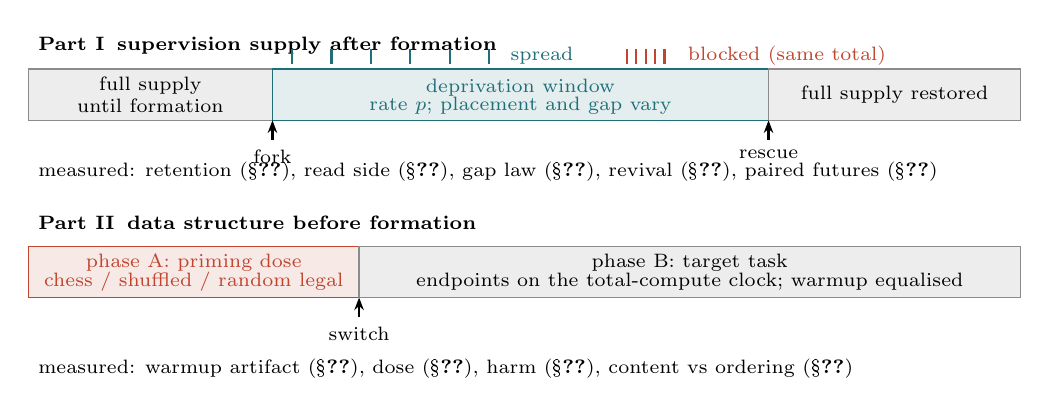
\begin{tikzpicture}[x=1cm, y=1cm, line width=0.5pt, font=\scriptsize,
                    >={Stealth[length=1.6mm]}]
% ---- Part I row: deprivation / supply ----
\node[anchor=west, font=\scriptsize\bfseries] at (0, 3.55) {Part I\enspace supervision supply after formation};
\draw[fill=black!7, draw=black!45] (0, 2.6) rectangle (3.1, 3.25);
\node[align=center] at (1.55, 2.925) {full supply\\ until formation};
\draw[fill=housetea!12, draw=housetea] (3.1, 2.6) rectangle (9.4, 3.25);
\node[housetea] at (6.25, 3.02) {deprivation window};
\node[housetea] at (6.25, 2.78) {rate $p$; placement and gap vary};
\draw[fill=black!7, draw=black!45] (9.4, 2.6) rectangle (12.6, 3.25);
\node at (11.0, 2.925) {full supply restored};
\draw[->, thick] (3.1, 2.35) -- (3.1, 2.6);
\node[anchor=north] at (3.1, 2.35) {fork};
\draw[->, thick] (9.4, 2.35) -- (9.4, 2.6);
\node[anchor=north] at (9.4, 2.35) {rescue};
% supervised-batch tick marks: spread vs blocked at identical totals
\foreach \x in {3.35, 3.85, 4.35, 4.85, 5.35, 5.85} \draw[housetea, line width=0.8pt] (\x, 3.32) -- (\x, 3.5);
\node[anchor=west, housetea] at (6.0, 3.42) {spread};
\foreach \x in {7.6, 7.72, 7.84, 7.96, 8.08} \draw[houseclay, line width=0.8pt] (\x, 3.32) -- (\x, 3.5);
\node[anchor=west, houseclay] at (8.25, 3.42) {blocked (same total)};
\node[anchor=west] at (0, 1.95) {measured: retention (\S\ref{sec:retention}), read side
(\S\ref{sec:readside}), gap law (\S\ref{sec:geometry}), revival (\S\ref{sec:revival}),
paired futures (\S\ref{sec:futures})};
% ---- Part II row: priming ----
\node[anchor=west, font=\scriptsize\bfseries] at (0, 1.30) {Part II\enspace data structure before formation};
\draw[fill=houseclay!12, draw=houseclay] (0, 0.35) rectangle (4.2, 1.0);
\node[houseclay] at (2.1, 0.79) {phase A: priming dose};
\node[houseclay] at (2.1, 0.55) {chess / shuffled / random legal};
\draw[fill=black!7, draw=black!45] (4.2, 0.35) rectangle (12.6, 1.0);
\node at (8.4, 0.79) {phase B: target task};
\node at (8.4, 0.55) {endpoints on the total-compute clock; warmup equalised};
\draw[->, thick] (4.2, 0.1) -- (4.2, 0.35);
\node[anchor=north] at (4.2, 0.1) {switch};
\node[anchor=west] at (0, -0.55) {measured: warmup artifact (\S\ref{sec:artifact}), dose
(\S\ref{sec:nopay}), harm (\S\ref{sec:harm}), content vs ordering (\S\ref{sec:strategy})};
\end{tikzpicture}
\caption{The two experimental designs, as forks of one training timeline. Part I forms the
capability, then manipulates only the rate and placement of supervised contact through a
deprivation window; tick marks illustrate two placements of an identical supervised total.
Part II manipulates only what the network trains on before the target task arrives, at
matched total compute and matched optimiser state. Sections are keyed to the phase they
measure.}
\label{fig:design}
\end{figure}

\section*{Part I\quad Supervision supply after formation}

\section{Retention: a small continuous rate suffices}
\label{sec:retention}

At $K=4$ on devaxis, zero supply through the deprivation window loses the capability in every run that had
it at the fork (\RetKfZero{} retained), while $p=0.03$ and above retains it in every run
(7/7 at each of $p=0.03$, $0.04$, $0.05$); the crossover sits between $p=0.01$
(\RetKfLow) and $p=0.03$, with \RetKfTwo{} at $p=0.02$. At $K=2$ the price is lower: total deprivation still retains
\RetKtZero, and $p=0.02$ retains \RetKtTwo{} (the \RetKtThree{} at $p=0.03$ sits within its
interval). The H100 program, under a stricter
held-throughout criterion, places full retention at $K=2$ between $p=0.05$ and $p=0.2$.
Retention is therefore threshold-shaped on both platforms, and load raises the price
(Figure~\ref{fig:retention}).

\begin{figure}[t]
\centering
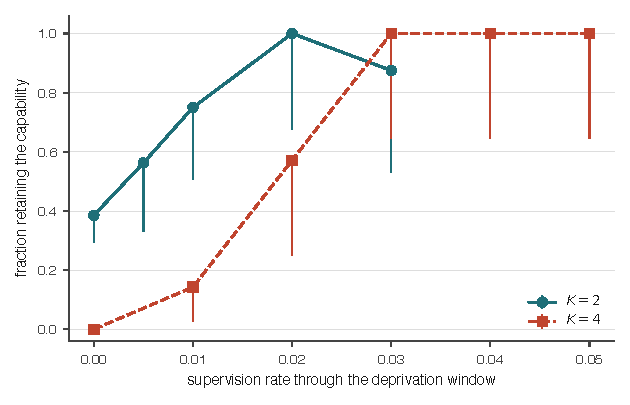
\includegraphics[width=0.667\linewidth]{figs_p456/p4_retention.pdf}
\caption{A small continuous rate retains the capability, and load raises the price. Fraction
of runs retaining the capability against the supervision rate held through the deprivation
window (devaxis platform; each point pools the runs at that rate that held the capability at
the fork, so denominators differ by point). Error bars are 95\% Wilson intervals on the
plotted fraction. $K=2$ retains \RetKtTwo{} at $p=0.02$ while $K=4$ requires $p=0.03$.
Generated by \texttt{analysis/make\_p456\_figs.py} from
\texttt{results/devaxis\_analyses.json}.}
\label{fig:retention}
\end{figure}

\section{The read side never goes}
\label{sec:readside}

Across every deprivation arm on the H100 platform, median end-of-run recap is 1.000 while
use-side accuracy sits at chance. The models are not damaged in general: held-out loss moves
little, and the recap stream is intact. The capability's content remains readable; what
degrades is its use. This is the observation that makes Part I coherent: a routing failure
can in principle be repaired cheaply, and a small maintenance signal can plausibly protect
routing while it could not plausibly re-teach content.

\section{Geometry: the maximum unsupervised gap is the controlling statistic}
\label{sec:geometry}

Three arms received the same residual supply ($p=0.01$ equivalent), with budgets verified to
differ by 0.00\% in a unit test before launch, differing only in placement: spread uniformly through the gap,
delivered as a burst at the start (front), or as a burst at the end (back). Spread re-formed
5/5; front 1/6; back 0/6 (Fisher: uniform vs front $p=0.0152$, uniform vs back $p=0.0022$).
Three readings were declared before the runs: continuous maintenance, recency, and
total-count. The data match continuous maintenance. Back placement, immediately before
rescue, is the worst arm, which rules out recency; the equality of totals rules out
total-count. The front--back comparison is uninformative at this $n$ ($p=1.0$).

The pre-registered follow-up (X14) filled the axis between these extremes
(Figure~\ref{fig:gaplaw}). Every arm delivers the same mean supply rate ($p=0.01$) and the
same supervised total, with totals verified to differ by 0.0000\% before launch; only the maximum
unsupervised gap between supervised batches moves, across a factor of \GapSpanFactor:
uniform $\approx$14 steps, periodic $\approx$99, clustered $\approx$990, contiguous blocks
$\approx$10{,}395. Re-formation falls monotonically along that axis: \GapCellUniform,
\GapCellPeriodic, \GapCellClustered, \GapCellBlocks{} (\GapCellUniformPct\%,
\GapCellPeriodicPct\%, \GapCellClusteredPct\%, \GapCellBlocksPct\%), and a logistic fit in
log gap puts the 50\% point near a gap of \GapFifty{} steps. Of the three readings declared
before any X14 run existed, the one that fires is near-every-step contact: both intermediate
arms fail. \GapIncomplete{} runs whose rescue phase had not completed when the platform
reached its fixed termination are excluded and counted, never scored as failures.

\begin{figure}[t]
\centering
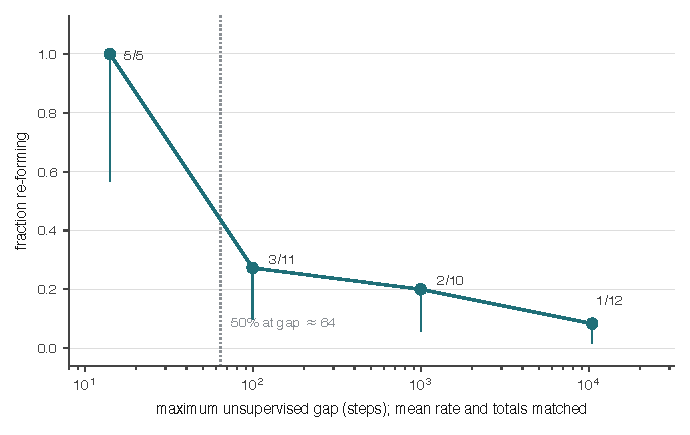
\includegraphics[width=0.730\linewidth]{figs_p456/p4_gaplaw.pdf}
\caption{The gap law. Re-formation against the maximum unsupervised gap between supervised
batches, at identical mean dose ($p=0.01$) and identical supervised totals (verified to
differ by 0.0000\% before launch). Point labels give re-formed/complete counts; error bars are 95\%
Wilson intervals; \GapIncomplete{} incomplete rescues are excluded and counted. The dotted
line marks the logistic fit's 50\% point at a gap of $\approx$\GapFifty{} steps. Generated
by \texttt{analysis/make\_p456\_figs.py} from \texttt{results/x14\_gap\_law.json}.}
\label{fig:gaplaw}
\end{figure}

\section{Revival: a higher threshold, and a wall at zero}
\label{sec:revival}

After a collapse, restoring full supply revives the capability only if some residual use
flowed through the gap. On the H100 platform the revival boundary sits between 0 and 1\% of
full supply: \RevZero{} re-form at zero (Fisher $p=0.0001$ against \RevOne{} at $p=0.01$),
\RevTwoTh{} at 0.002, \RevFiveTh{} at 0.005, \RevOne{} from 0.01 up. At true zero the loss
is irreversible in this budget: six runs each received at least $8\times$ their original
formation compute at full supply and 0/6 re-formed, with recap still at 1.000. A collapsed
network is worse at rebuilding this task than a fresh initialisation.

The devaxis revival experiments, at higher load and different windows, place their boundary
near 20\% of full supply (0/24 at rates $\le 0.05$ vs 4/8 at 0.20, Fisher $p=0.0019$).
Retention replicates cleanly across the platforms; the revival threshold does not transfer
across load and protocol, and its dependence on $K$ is open.

\section{Same behaviour, different futures}
\label{sec:futures}

The paired-fork experiment on devaxis makes the maintenance variable visible by hiding it
from behaviour. Models that received a trickle of supply through the window ($p=0.005$, about
fifty supervised step-equivalents over ten thousand steps) and models that received none are
indistinguishable at rescue time: both sit at chance on the use side, both read perfectly.
Their futures differ: 31/40 vs 18/40 recover under full restore (McNemar $p=0.0072$;
log-rank $p=0.0146$), and on the same eight seeds the paired contrast is 8/8 vs 1/8 (McNemar
$p=0.0156$). Plasticity itself declines with time deprived: a paired probe finds decline in
15/16 parent runs (exact sign test $p=0.0005$). An earlier pooled version of the trickle result
(``24/24, $p=2\times10^{-6}$'') was withdrawn when per-dose checks showed two of its arms
had never collapsed; the surviving claim is the paired one just stated.

\section{The cost of load}
\label{sec:costload}

Median time to first formation grows as a power of $K$: $t \approx
\TimeLawHCoef\,K^{\TimeLawHExp}$ ($R^2=\TimeLawHRsq$) on the H100 platform and $t \approx
\TimeLawDCoef\,K^{\TimeLawDExp}$ ($R^2=\TimeLawDRsq$) on devaxis, fits made independently,
the first before the second corpus was examined. The form replicates; the exponent does not
pin down (the devaxis $K{=}8$ cell holds two runs, and removing it moves the exponent to
\TimeLawExpNoKeight), and both are lower bounds because runs that never emerged are censored
out. Seed matters far beyond chance: across 24 seeds the variance of emergence rate is
$\SeedOverdisp\times$ the binomial expectation, so per-seed comparisons must be paired. The
companion capacity manuscript reports this law's figure and its consequences for budgeting
in-context memory.

\section*{Part II\quad Data structure before formation}

\section{The artifact}
\label{sec:artifact}

With no priming at all, the baseline's median time-to-threshold is 28{,}250 steps with a
500-step LR warmup and 6{,}750 without it: a factor of 4.19, Mann--Whitney
$p=1.9\times10^{-7}$, with 29 of 30 warmup-free runs faster than every warmup run. An
earlier statement that the distributions were disjoint was retracted when one warmup-free
run crossed at its budget cap; the effect is unchanged.

Against the warmup-handicapped baseline, every substrate helps by roughly the size of the
handicap, and the specificity gate fails: shuffled chess helps too ($p<0.0001$). The
low-dose transfer result is therefore an optimiser artifact; the priming data played no part
in it.

\section{Does any dose pay?}
\label{sec:nopay}

With warmup equalised on all arms including the baseline (which then crosses in a median of
5{,}875 steps), chess priming at doses 2{,}000 and 5{,}000 is directionally worse than no
priming, significant on the time-to-event test that uses censored runs ($p=0.037$, $0.026$)
and not significant on crossing rate at $n=6$. Three baseline pools appear in this part,
all on the warmup-free protocol: this equalised pool (median 5{,}875), the re-derivation's
pool (median \WuFastMed, $n=\WuFastN$), and the replication's pooled baseline (median
\DzBaseMed, $n=\DzBaseN$); the arithmetic below uses the first. Three outcomes were declared before launch;
on these doses the one that fired is ``no dose pays.'' A later re-derivation from raw
records (Section~\ref{sec:rederive}) adds nuance at the smallest dose: on the total clock,
chess at dose 250 is directionally faster than the warmup-free baseline (5{,}500 vs
6{,}750, $p=0.063$, $n=9$), and on the phase-B clock it is faster at $p=0.025$ under the
rule declared for that analysis, which does not survive correction across the five doses
tested ($p=0.125$). That cell was then settled by a pre-registered replication: 20 new seeds
of chess at dose 250, 20 of shuffled chess, and 6 contemporaneous baselines, with the
endpoint, the single test, and three verdict gates fixed in a registration uploaded before
launch and the verdict script committed before any run finished.

The verdict is negative. Chess at dose 250 crosses \DzChessCross/\DzChessN{} with median
\DzChessMed{} vs \DzBaseMed{} for the pooled baseline ($n=\DzBaseN$, \DzBaseCross/\DzBaseN{}
crossing); Mann--Whitney with censored runs ranked worst gives $p=\DzPChess$, and the
phase-B clock agrees ($p=0.41$). The direction favours priming; the magnitude does not
survive $n=\DzChessN$. The specificity gate returned a result of its own: shuffled chess at
dose 250 is significantly slower than baseline (median \DzShufMed, \DzShufCens/20 censored,
$p=\DzPShuf$ two-sided), the pre-specified test firing in the unanticipated direction. At
this dose the structure-free control hurts.

Arithmetic closes the question for this target: the baseline needs 5{,}875 steps in total,
so a 2{,}000-step dose spends 34\% of the entire requirement on priming. A target on which
priming could pay would need a baseline requirement many times the dose; neither alternative
target in the same experimental block qualifies (one crosses 0/5, the other has no baseline), so we mark the
compute question unanswerable on this task family rather than answered in the negative
beyond the doses measured.

\section{What survives: harm from unstructured data}
\label{sec:harm}

Chess and shuffled chess have identical token statistics (measured total-variation distance
0.000000); shuffling destroys the game structure. Below a dose of 5{,}000 steps the two arms
are indistinguishable on crossing rate. At and above it they separate sharply
(Figure~\ref{fig:harm}): in the raw-record accounting that the figure draws, dose 20{,}000
crosses \HarmChessTwenty{} under structured priming and \HarmShufTwenty{} under
structure-free priming (exact Fisher $p=\HarmPTwenty$; the campaign's own block accounting reads 20/24
vs 0/9, pooled 36/39 vs 1/16, the same dissociation). Both arms pay identical compute and
arrive equally warmed, so neither confound applies. Because the warmup-500 unprimed
baseline, the stratum these arms belong to, crosses at \WuSlowCross/\WuSlowN, the result is asymmetric: a large dose of
unstructured data destroys the ability to learn the target, and structured data of the same
statistics does not. Nothing in the program shows structure adding anything over no priming
at all. The pre-registered replication at dose 250 (Section~\ref{sec:nopay}) moves the harm
boundary down: on the time-to-threshold clock, structure-free priming is already slower than
no priming at the smallest dose measured ($p=\DzPShuf$), although crossing rate stays high
(\DzShufCross/20). The same dissociation appears on the speed axis at matched optimiser
state: after equal doses, the post-priming phase is $\SpeedRatio\times$ longer after
structure-free priming than after structured priming (Section~\ref{sec:rederive}).

\begin{figure}[t]
\centering
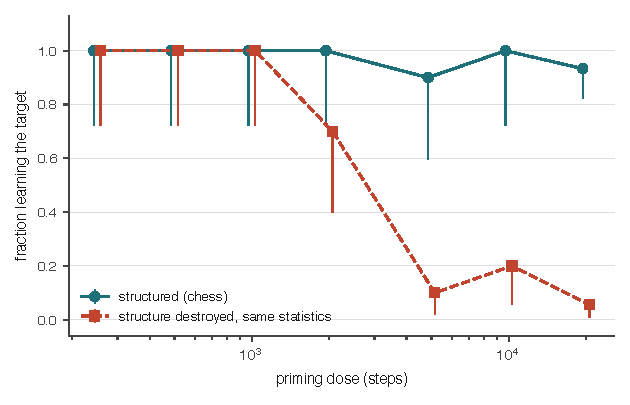
\includegraphics[width=0.667\linewidth]{figs_p456/p5_harm.pdf}
\caption{Structure in the priming data decides whether the target remains learnable.
Fraction of runs learning the target task after priming, against priming dose, at warmup 500
on both arms. The two substrates have identical token statistics (measured total-variation
distance 0.000000); below dose 5{,}000 the arms are indistinguishable on crossing rate, and
above it structure-destroyed priming nearly abolishes learning (\HarmShufTwenty{} at dose
20{,}000) while structured priming preserves it (\HarmChessTwenty). Error bars are 95\%
Wilson intervals; points are dodged horizontally by 3\% so coincident values stay visible.
Generated by \texttt{analysis/make\_p456\_figs.py} from
\texttt{results/h100\_reanalysis.json} (the raw-record re-derivation).}
\label{fig:harm}
\end{figure}

\section{Strategy is null; ordering is not}
\label{sec:strategy}

Within structured priming, content does not matter here: random legal chess games match real
games (pooled 148/169 vs 60/64, Fisher $p=0.24$; log-rank $p=0.26$). Legality and board
state carry whatever the substrate carries. Ordering, however, matters at a fixed token
multiset: cyclic presentation beats iid at $n=24$ ($\chi^2=7.47$, $p=0.0063$, Holm
$0.0189$), a result that was a null at $n=8$ and resolved under the powered replication.

\section{Independent re-derivation}
\label{sec:rederive}

As a check on Part II's conclusions and the Part I revival table, every headline number was re-derived from the raw run
JSONs by a script whose definitions and decision rules were fixed before computation
(\path{analysis/h100_reanalysis.py}; 651 priming and 230 maintenance runs parsed). The
warmup handicap reproduces (\WuSlowMed{} vs \WuFastMed{} median, ratio \WuRatio,
$p=\WuP$). The artifact test reproduces decisively: at warmup 500 and doses 250--1{,}000,
chess saves \SaveChessLo--\SaveChessHi k steps against the cold baseline while shuffled
chess saves \SaveShufLo--\SaveShufHi k and random legal games save
\SaveRandLo--\SaveRandHi k; the control saves what the treatment saves. The strategy null
reproduces (\StratChessR{} vs \StratRandR, $p=\StratP$). One effect is sharpened: at matched
warmup and dose 5{,}000, the post-priming phase takes \SpeedChessB{} steps after chess and
\SpeedShufB{} after shuffled chess; against the warmup-matched baseline the shuffled arm is
slower ($p=\SpeedShufP$) while the chess arm is not ($p=\SpeedChessP$), so structure changes
learning speed, not only learnability. The dose-250 signal this re-derivation surfaced was subsequently tested
and closed by the pre-registered replication reported in Section~\ref{sec:nopay}.

\section{Consequences}
\label{sec:consequences}

Part I prices a training decision that is currently made blind, and the price asymmetry is
extreme. Keeping a formed capability
alive costs 1--3\% of full supervision under the devaxis retention criterion (the stricter
held-throughout criterion prices it higher); the deciding signal in the paired-fork experiment
is about fifty supervised step-equivalents spread across ten thousand steps. Letting the
capability collapse and curing it afterward costs an
order of magnitude more, and past a boundary it cannot be cured at all: at true zero the
collapsed network re-forms in 0/6 runs given at least $8\times$ its own formation compute,
worse than a fresh initialisation, so beyond the wall the economical move is retraining, not
rescue. Because the deciding
variable is invisible to behavioural monitoring, continual-training pipelines that watch
only task metrics will systematically miss the moment intervention is cheap. The read/use
split supplies the monitoring target: track whether stored content is still being routed,
not whether it is still stored. And the placement result converts schedule design from
folklore into a measured constraint: supervision budgeted for retention must be spread
through the stream at fine granularity, because banking it in a block forfeits it; on this
platform, unsupervised gaps beyond a few tens of steps already forfeit the majority of
re-formation.

Part II is directly actionable in two places, and it too is a budget statement: priming is
paid for out of the target-task budget, a 2{,}000-step dose already spends 34\% of the entire
baseline requirement at this scale, no measured dose earns that spend back, and a large
structure-free dose destroys the investment outright by leaving the target unlearnable. For
data curation: structural integrity of
early training data is a gate on later learnability, at fixed token statistics, so filtering
pipelines that score data by distributional features alone measure the wrong thing. For
evaluation practice: any curriculum or pre-pretraining comparison whose baseline starts cold
inherits a confound the size of the entire claimed effect, and the warmup-matched protocol
here removes it for the cost of one flag. The dissociation between content (irrelevant) and
structure and order (decisive) also narrows the mechanistic search space for why early data
shapes later learning.

Stated in tokens, the same economics sharpen. Tokens per step is batch size times sequence
length, recorded in every raw run record, so each step count above has an exact token
equivalent. The
deciding trickle in the paired-fork experiment is \TokTrickle{}M supervised tokens inside a
\TokWindow{}M-token window: \TokTricklePct\% of throughput decides whether the capability
survives. The gap ceiling sits near \TokGapFifty{}M unsupervised tokens between contacts. On
the priming side, the target task costs \TokBaseReqLo{}--\TokBaseReqHi{}M tokens to learn
under the two accountings; the structure-free dose that removes learnability is
\TokHarmDose{}M tokens, roughly three times that requirement; and the warmup default alone
costs \TokWuWaste{}M tokens per run, \TokWuWasteMult$\times$ the task's own requirement.
The conversion is derived per pool from the raw run records by
\texttt{analysis/token\_costs.py}.

The joint lesson is about instrumentation. The two levers this paper measures, supervised
contact after formation and data structure before it, are exactly the levers that standard
pipeline instruments do not read: behavioural monitoring cannot see the supply variable, and
distributional filters cannot see structure.

\section{Related work}
\label{sec:related}

The maintenance question has a continual-pretraining literature whose instrument is the
replay fraction. Ibrahim et al.\ \cite{ibrahim2024} show that learning-rate re-warming, re-decaying, and
replay of previous data together match full retraining from scratch when continually
pretraining large models; the replay percentages they carry forward are chosen for a
favourable loss--compute tradeoff, not measured as thresholds. Bethune et al.\ \cite{bethune2025} measure
forgetting during finetuning and find that injecting as little as 1\% of pretraining data
shields the model from forgetting the pretraining set. Both results price the fraction of
old data; neither varies its placement at a fixed budget. The gap law of
Section~\ref{sec:geometry} is that missing measurement on this platform: at matched rate
and totals, the maximum unsupervised gap is the controlling statistic. On the read/use
split, Zheng et al.\ \cite{zheng2025} argue from task sequences that performance drops in continual
learning often reflect a decline in task alignment rather than true knowledge loss; the
recap-vs-query dissociation here is the same distinction with the storage side pinned at
1.000, and Part I builds the supply economics on top of it.

Plasticity loss \cite{dohare2023, lyle2023} names the degradation of the ability to learn
new things under continued training. Dong \cite{dong2026} locates a formation deadline on
Pythia-family models: the delay to learn a withheld capability grows with waiting until,
past a critical step, it never ignites, while validation loss falls smoothly throughout,
and re-initialising the query--key attention slices restores learnability. That result
concerns capabilities not yet formed; Part I measures the formed side, where the wall is
indexed by deprivation after formation and the collapsed network rebuilds the task worse
than a fresh initialisation. The two deadlines bound a capability's life from opposite
ends.

On the priming side, the closest design is pre-pretraining on formal languages
\cite{hu2025}, at 1B parameters: hierarchical formal languages transfer to natural
language, random strings are harmful relative to no pre-pretraining, $n$-gram-matched
``metamer'' controls transfer less than the structured original, and there is an optimal
dose past which more pre-pretraining transfers less. Their metamer arm is compared with its
structured original; the design here closes the remaining cell, statistics-matched data
against the no-priming baseline, and moves the outcome from validation loss to whether the
target is learnable at all (Section~\ref{sec:harm}). Two adjacent results point the other
way and mark the scope boundary. In vision, early deficits that leave low-level statistics
unchanged have no lasting effect \cite{achille2019}; the harmful arm here preserves unigram
statistics and destroys sequential structure, so the vision rule does not transfer to this
setting. In language models, delayed second-language exposure produces no critical-period
effect \cite{constantinescu2024}; that manipulation varies when data arrives, not what its
structure is, and the two findings are compatible. On the artifact, Porian et al.\ \cite{porian2024} show
that a constant-length warmup default is too long for small models and inflates estimated
optimal token counts, enough to account for part of the disagreement between published
scaling laws; Section~\ref{sec:artifact} prices the same class of default for a single run,
a factor of \WuRatio{} on the baseline's own clock.

\section{Scope}
\label{sec:limits}

The measurements are on 1.3M--5M-parameter transformers and synthetic sequence tasks of one
family, the regime where hundreds of runs per cell are affordable and threshold structure is
resolvable. Extending both levers to language-model pretraining at scale is the natural next
measurement, and the companion capacity work shows the regimes can differ by large factors. In Part I, the revival threshold disagrees across platforms and loads; the
learning-time exponent rests on few loads; ``continuous maintenance'' names a schedule
property, and the mechanism behind it is open. The pre-registered X14 experiment
(Section~\ref{sec:geometry}) localises the controlling statistic to the placement axis, with
contact required at near-every-step granularity, but its per-arm $n$ is 5--12,
\GapIncomplete{} incomplete rescues are excluded, and the 50\%-point estimate of \GapFifty{}
steps is a fit; the boundary itself is unmeasured between gaps of 14 and 99. All causal
claims concern the supply manipulation; no claim is made about internal representations
beyond the read/use split that the two accuracies measure. In Part II, the harm result has
4--24 runs per cell under the block accounting (up to 45 under the pooled raw-record
accounting); the compute question is bounded but not settled, since doses between 250 and
20{,}000 were measured on one target family whose baseline requirement leaves little
headroom; the strategy null is a failure to detect at $n$ of tens, with the pooled contrast
reported. The developmental-state appendix is observational and carries an unresolved metric
confound by construction.

\section*{Reproducibility Statement}
Code, data, and the paper source are public at
\begin{center}
\url{https://github.com/RavulapalliManas/paper-training-history}
\end{center}
\noindent Every macro-backed number in the prose regenerates from committed result files:
running \path{analysis/make_numbers.py} rebuilds \texttt{numbers.tex} byte-for-byte
from \texttt{results/}. Each committed result file ships with its generator, named
\texttt{results/<name>.json} and \texttt{analysis/<name>.py}:
\begin{itemize}
\item retention, revival, and futures cells: \texttt{devaxis\_analyses};
\item the pre-registered gap-law experiment: \texttt{x14\_gap\_law};
\item the raw-record priming re-derivation: \texttt{h100\_reanalysis};
\item the pre-registered dose-250 replication: \texttt{d250\_verdict};
\item the token conversion: \texttt{token\_costs}.
\end{itemize}
Figures are drawn by \path{analysis/make_p456_figs.py} from the committed files only.
The raw run records of the \DevaxisRuns{} Trainium and 985 H100 runs live in the two
training codebases and are available on request; the scripts above state exactly how each
committed file was derived from them.

\begin{thebibliography}{9}
\setlength{\itemsep}{1pt}\small

\bibitem{achille2019}
A.~Achille, M.~Rovere, and S.~Soatto. Critical learning periods in deep neural networks.
2019. arXiv:1711.08856.

\bibitem{bengio2009}
Y.~Bengio, J.~Louradour, R.~Collobert, and J.~Weston. Curriculum learning. \emph{ICML}, 2009.

\bibitem{bethune2025}
L.~Bethune, D.~Grangier, D.~Busbridge, E.~Gualdoni, M.~Cuturi, and P.~Ablin. Scaling laws
for forgetting during finetuning with pretraining data injection. 2025. arXiv:2502.06042.

\bibitem{constantinescu2024}
I.~Constantinescu, T.~Pimentel, R.~Cotterell, and A.~Warstadt. Investigating critical period
effects in language acquisition through neural language models. \emph{TACL}, 2024.
arXiv:2407.19325.

\bibitem{dohare2023}
S.~Dohare, J.~F.~Hernandez-Garcia, P.~Rahman, A.~R.~Mahmood, and R.~S.~Sutton. Maintaining
plasticity in deep continual learning. 2023. arXiv:2306.13812.

\bibitem{dong2026}
L.~Dong. The kinetics of training: a driven-nucleation rate law for emergence, plasticity
loss, and circuit control in language models. 2026. arXiv:2607.27281.

\bibitem{french1999}
R.~M.~French. Catastrophic forgetting in connectionist networks. \emph{Trends in Cognitive
Sciences}, 3(4):128--135, 1999.

\bibitem{goyal2017}
P.~Goyal, P.~Doll\'ar, R.~Girshick, et al. Accurate, large minibatch SGD: training ImageNet
in 1 hour. 2017. arXiv:1706.02677.

\bibitem{hu2025}
M.~Y.~Hu, J.~Petty, C.~Shi, W.~Merrill, and T.~Linzen. Between circuits and Chomsky:
pre-pretraining on formal languages imparts linguistic biases. \emph{ACL}, 2025.
arXiv:2502.19249.

\bibitem{ibrahim2024}
A.~Ibrahim, B.~Th\'erien, K.~Gupta, M.~L.~Richter, Q.~Anthony, T.~Lesort, E.~Belilovsky,
and I.~Rish. Simple and scalable strategies to continually pre-train large language models.
2024. arXiv:2403.08763.

\bibitem{kirkpatrick2017}
J.~Kirkpatrick, R.~Pascanu, N.~Rabinowitz, et al. Overcoming catastrophic forgetting in
neural networks. \emph{PNAS}, 114(13):3521--3526, 2017. arXiv:1612.00796.

\bibitem{lyle2023}
C.~Lyle, Z.~Zheng, E.~Nikishin, B.~Avila~Pires, R.~Pascanu, and W.~Dabney. Understanding
plasticity in neural networks. \emph{ICML}, 2023. arXiv:2303.01486.

\bibitem{mccloskey1989}
M.~McCloskey and N.~J.~Cohen. Catastrophic interference in connectionist networks: the
sequential learning problem. \emph{Psychology of Learning and Motivation}, 24:109--165, 1989.

\bibitem{papadimitriou2020}
I.~Papadimitriou and D.~Jurafsky. Learning music helps you read: using transfer to study
linguistic structure in language models. \emph{EMNLP}, 2020. arXiv:2004.14601.

\bibitem{porian2024}
T.~Porian, M.~Wortsman, J.~Jitsev, L.~Schmidt, and Y.~Carmon. Resolving discrepancies in
compute-optimal scaling of language models. \emph{NeurIPS}, 2024. arXiv:2406.19146.

\bibitem{schaeffer2023}
R.~Schaeffer, B.~Miranda, and S.~Koyejo. Are emergent abilities of large language models a
mirage? \emph{NeurIPS}, 2023. arXiv:2304.15004.

\bibitem{wu2021}
Y.~Wu, M.~Rabe, W.~Li, J.~Ba, R.~Grosse, and C.~Szegedy. LIME: learning inductive bias for
primitives of mathematical reasoning. \emph{ICML}, 2021. arXiv:2101.06223.

\bibitem{zheng2025}
J.~Zheng, X.~Cai, S.~Qiu, and Q.~Ma. Spurious forgetting in continual learning of language
models. \emph{ICLR}, 2025. arXiv:2501.13453.

\end{thebibliography}

\appendix
\section{Provenance}
\label{sec:provenance}

Retention scoring requires a guard, stated here because its absence produced a wrong table
first: a run that never had the capability at the fork cannot lose it, and counting such
runs as failures produced the impossible cell ``full supply, 0/36 retained'' before the
condition was added.

{\sloppy
Every number above traces to a committed document or script. D = the devaxis results
document (\path{research/devaxis-trainium/RESULTS_2026-08-10.md}, regenerated from raw run
JSONs by \path{analysis/results_tables.py}); F = the H100 farm document
(\path{ALL_RESULTS_farm.md}, generated 2026-08-10 by \path{analysis/all_results.py}); T =
the Tier-0 closure report (\path{TIER0_REPORT_farm.md}); C = the clocks snapshot
(\path{RESULTS.md}, 2026-08-09); P = the pre-registered dose-250 replication
(\path{PREREG_d250_replication.md}, uploaded to S3 before launch; 46 runs; verdict in
\path{results/d250_verdict.json}, script committed before the data existed); R = recomputed
in this repository by the named script over committed JSONs, with headline values emitted as
macros by \path{analysis/make_numbers.py} and staleness-gated by \path{analysis/verify.py}.
The farm documents live under \path{research/emergence-clocks-2026-08/} and in S3.
Architecture and optimiser configurations beyond the quantities the claims use live in the
campaign documents and per-run records named here, not in this paper.\par}

\begin{center}
\footnotesize
\begin{tabular}{ll}
\hline
claim & source \\
\hline
retention cells at $K{=}4$ and $K{=}2$; H100 held-throughout table & R (\texttt{devaxis\_analyses.py}); F \S2 \\
recap 1.000 and stable held-out loss through every collapse & F \S2, \S3 \\
geometry 5/5 / 1/6 / 0/6, budgets matched 0.00\% & F \S4 \\
X14 gap axis and gap50 & R (\texttt{x14\_gap\_law.py}) \\
revival dose table, boundary 0--0.01 & R (\texttt{h100\_reanalysis.py}); F \S3b \\
irreversibility 0/6 at $8\times$ budget & F \S3a \\
31/40 vs 18/40; 8/8 vs 1/8; plasticity decline 15/16 & D \\
withdrawn pooled trickle claim & D (corrections section) \\
learning-time fits and exponent sensitivity & R (\texttt{extra\_analyses.py}, \texttt{devaxis\_analyses.py}) \\
seed overdispersion $\SeedOverdisp\times$ & R (\texttt{devaxis\_analyses.py}) \\
warmup 28{,}250 vs 6{,}750, 4.19$\times$, $p=1.9\times10^{-7}$ & T R0.4a \\
retraction of the no-overlap phrasing & T R0.4a \\
specificity failure under crippled baseline & T R0.4a \\
no dose pays; directional harm at 2k/5k & T R0.4d (X15) \\
harm dissociation, block accounting, TV distance 0.000000 & F \S6b \\
harm dissociation, raw-record accounting (figure) & R (\texttt{h100\_reanalysis.py}) \\
survivor-conditioning correction & F \S6a, \S8b \\
strategy null 148/169 vs 60/64 & T R0.4c \\
cyclic vs iid, $n=24$ & C \S6 (Program E) \\
re-derivation: warmup, artifact, strategy, speed effect & R (\texttt{h100\_reanalysis.py}) \\
dose-250 acceleration signal and its Holm status & R (\texttt{h100\_reanalysis.py}) \\
dose-250 replication verdict, shuffle slowdown & P (\texttt{d250\_verdict.py}) \\
farm run totals and the 651/230 parse split & F; R (\texttt{h100\_reanalysis.py}) \\
rung occupancy, mid-rung share, metric caveat & F \S1a--1c, \S8a \\
mirage control, 963 measurements & C \S3 (X1) \\
\hline
\end{tabular}
\end{center}

\section{Developmental-state observations}
\label{sec:states}

The H100 platform tracked per-register mastery during formation of a $K=6$ binding. Runs
occupy rung 0 (61 of 85), rung 1 (20), or rung 6 (4) of the mastery ladder; rungs 2--5 are
empty, and across 202{,}148 evaluations the middle rungs hold 0.07\%. A run masters one
register, waits, then takes the remaining five together. The campaign's own caveat is
retained here: the scalar accuracy is exactly the item-weighted mean of the per-slot vector,
so ``the ladder is discrete'' and ``the slots master together'' describe a single
measurement, and the state-count test that would separate internal states from a metric
consequence was specified and not run. The mirage control, run here against the metric
artifact that \cite{schaeffer2023} describe, does
establish that emergence itself is not a thresholding artifact on this platform:
unthresholded metrics
complete their rise inside the accuracy jump window across 963 (run, metric) measurements.

\end{document}
